\pagenumbering{gobble}
\maketitle
\newpage
\pagenumbering{roman}
\setcounter{page}{1}

\clearpage

\cleardoublepage
\phantomsection

\subpdfbookmark{Sadržaj}{name}
\tableofcontents

\clearpage
\pagenumbering{arabic}

\chapter{Uvod}

\section{Greške}

Greške su neizbježne, prilikom izračuna je cilj smanjiti njihov utjecaj na krajnji rezultat.

\subsection{Vrste grešaka}

\begin{itemize}
    \item \textbf{Greška modela} nastaje zamjenom nekog složenog sustava ili procesa jednostavnijim.
    \begin{itemize}
        \item Neki sustavi su pre složeni da bi se opisali i riješili poznatim matematičkim alatima.
        \item Primjer: otpor zraka u balistici
    \end{itemize}
    \item \textbf{Greška metode} nastaje zamjenom procesa (obično beskonačnog) konačnom aproksimacijom.
    \begin{itemize}
        \item Primjer: određivanje sume beskonačnog reda
    \end{itemize}
    \item \textbf{Greška diskretizacije} nastaje kada umjesto podataka koje nije moguće potpuno ispravno pohraniti ili predstaviti koristimo njima bliske podatke (aproksimacije).
    \begin{itemize}
        \item Primjeri:
        \begin{itemize}
            \item $\pi, e, \dots$
            \item Zamjena kontinuuma konačnim diskretnim skupom
            \item Zamjena beskonačno male veličine s malom, konkretnom veličinom
        \end{itemize}
    \end{itemize}
    \item \textbf{Ulazna pogreška} nastaje zbog pogrešaka u ulaznim podacima nastalih prethodnom obradom podataka ili greškom mjerenja.
    \begin{itemize}
        \item Primjer: akceleracija sile teže.
    \end{itemize}
\end{itemize}

Zaokruživanjem ili odbacivanjem decimala u prikazu broja a u računalu dobivamo aproksimaciju realnog broja (\textit{engl.} floating point approximation) od $a$ koju označavamo s fl$(a)$ i za koju vrijedi:

$$
\text{fl}(a) = a(1+\varepsilon)
$$

gdje je $\varepsilon$ \textbf{greška aproksimacija}.

\newpage

\subsection{Zapis realnog broja u računalu}

Za zapis realnih brojeva se generalno koristi IEEE-754 standard.

U IEEE-754 standardu su brojevi pohranjeni s tri komponente:

\begin{center}
    \begin{tabular}{|l|l|}
        \hline
        Ime&Opis\\
        \hline
        Predznak&\verb|1| ako se radi o negativnom broju\\
        Eksponent&eksponent na bazi pohranjenog broja\\
        Mantisa/realni dio&decimalni dio realnog broja\\
        \hline
    \end{tabular}
\end{center}

Prilikom pohrane se podrazumijeva da mantisa ima prefiksni bit \verb|1| koji se ne piše jer nema smisla pohraniti broj s vodećim nulama.

IEEE-754 navodi raspored bitova za realne brojeve različitih veličina. Predznak je uvijek veličine jednog bita, a ostali karakteristike su navedene u sljedećoj tablici:

\begin{center}
    \begin{tabular}{l|c|c|c|c|c}
        Podatak&binary16&binary32&binary64&binary128&binary256\\
        \hline
        \hline
        Eksponent&5b&8b&11b&15b&19b\\
        Mantisa&10b&23b&52b&122b&236b\\
        Ukupna veličina&16b&32b&64b&128b&256b\\
        \hline
        \hline
        $ulp^*$&$2^{-11}$&$2^{-24}$&$2^{-53}$&$2^{-123}$&$2^{-237}$\\
        \hline
        \hline
        $exp_{min}$&-14&-126&-1022&-16383&-262142\\
        $exp_{max}$&+15&+127&+1023&+16384&+262143\\
        \hline
        \hline
        $val_{min}$ (normalan)&$6.10\cdot10^{-5}$&$1.18\cdot10^{-38}$&$2.23\cdot10^{-308}$&$3.36\cdot10^{-4932}$&$2.48\cdot10^{-78913}$\\
        $val_{min}$ (subnormalan$^{**}$)&$5.96\cdot10^{-8}$&$1.40\cdot10^{-45}$&$4.94\cdot10^{-324}$&$6.48\cdot10^{-4966}$&$2.25\cdot10^{-78984}$\\
        $val_{max}$&65504&$3.40\cdot10^{38}$&$1.80\cdot10^{308}$&$1.19\cdot10^{4932}$&$1.61\cdot10^{78193}$\\
    \end{tabular}
\end{center}

\begin{itemize}[label={}]
    \item * \textbf{ulp}: jedinična strojna greška, također se zove i \textit{strojni epsilon}.
    \item ** subnormalne IEEE-754 vrijednosti su spremljene manjom decimalnom preciznošću, tj. uz veću jediničnu strojnu grešku
\end{itemize}

\subsubsection{Posebne vrijednosti}

IEEE-754 brojevi također imaju posebne vrijednosti kojima simboliziraju da se prilikom operacije dogodilo prekoračenje minimalne/maksimalne vrijednosti (\verb|+inf| i \verb|-inf|), te kada je provedena nevaljana operacija nad brojem \verb|NaN| poput dijeljenja s nulom.

\begin{center}
    \begin{tabular}{ |c|c|c|c| } 
        \hline
        Ime &
        \multicolumn{3}{|c|}{Binarni zapis}\\
        \hline
        \verb|+inf|&\verb|0|&\verb|1|\dots\verb|1|&\verb|0|\dots\verb|0|\\
        \hline
        \verb|-inf|&\verb|1|&\verb|1|\dots\verb|1|&\verb|0|\dots\verb|0|\\
        \hline
        \hline
        \verb|NaN|&\verb|_|&\verb|1|\dots\verb|1|&\verb|_|\dots\verb|_|\\
        \hline
    \end{tabular}
\end{center}

Zbog toga što \verb|NaN| može biti predstavljen s mnogo različitih binarnih kombinacija, jednačenje realnih brojeva na računalu nije smisleno rješivo. Različiti programski jezici se nose s tim problemom na različite načine:

\begin{itemize}
    \item tretiraju sve \verb|NaN| vrijednosti kao istu,
    \item tretiraju svaku (čak i one čiji binarni zapisi se podudaraju) kao različitu,
    \item bacaju grešku prilikom usporedbe,
    \item imaju koncepte \textit{djelomično jednačivih/usporedivih} vrijednosti.
\end{itemize}

\section{Apsolutna i relativna greška}

Razliku $a-a^*$ između \textit{stvarne veličine} a i \textit{njene aproksimacije} $a^*$ nazivamo \textbf{greška aproksimacije}. Apsolutnu vrijednost greške aproksimacije nazivamo \textbf{apsolutna greška aproksimacije} i označavamo je s $\Delta a^*$. Vrijedi:

$$
\Delta a^* = |a-a^*|
$$

Omjer između apsolutne greške $\Delta a^*$ i apsolutne vrijednosti $|a|$ nazivamo \textbf{relativna greška} i označavamo je s $\delta a^*$. Vrijedi:

$$
\delta a^* = \frac{\Delta a^*}{|a|},\qquad a\neq0
$$

S obzirom da u praksi često nije poznata točna vrijednost $a$, koristi se \textbf{aproksimacija relativne greške}:

$$
\delta a^* \approx \frac{\Delta a^*}{|a^*|},\qquad a\neq0
$$

\begin{itemize}
    \item Redoslijed izvršavanja operacija na računalu je bitan jer utječe na veličinu greške zbog ograničene pohrane decimalnih brojeva (floating point error).
    \begin{itemize}
        \item Zbrajanje i množenje nisu asocijativni
        \item Množenje prema zbrajanju nije distributivno
    \end{itemize}
\end{itemize}

\subsection{Katastrofalno kraćenje}

Oduzimanje brojeva $x$ i $y$ koji su istog predzanaka može izazvati proizvoljno velike greške kada je $|x-y| \ll |x|,|y|$

Za katastrofalno kraćenje vrijedi:

\begin{gather*}
(x-y)(1+\varepsilon) = x(1+\varepsilon_x) - y(1+\varepsilon_y)\\
|\varepsilon| \leq \left|\frac{x}{x-y}\right| |\varepsilon_x| + \left|\frac{y}{x-y}\right| |\varepsilon_y|
\end{gather*}

Jedna od metoda izbjegavanja kraćenja je racionalizacija korijenu koja daje puno točniji rezultat za $x_1$:
$$
    x_1=-p+\sqrt{p^2+q}\cdot\frac{-p-\sqrt{p^2+q}}{-p-\sqrt{p^2+2}}=\frac{q}{p+\sqrt{p^2+q}}
$$


\chapter{Metode interpolacije}

\section{Metode interpolacije}

Interpolacija je postupak kojim od zadanih točaka neke funkcije $f(x)$ dolazimo
do funkcije $g(x)$ koja prolazi tim točkama i \textit{blisko prati} $f(x)$.

Interpolacija uključuje pogreške mjerenja tako da je netočno reči $g(x) = f(x)$,
no polinom ili po dijelovima funkcija koju dobijemo interpolacijom će dati
dobar uvid u međuvrijednosti zadanih točaka.

\begin{center}
    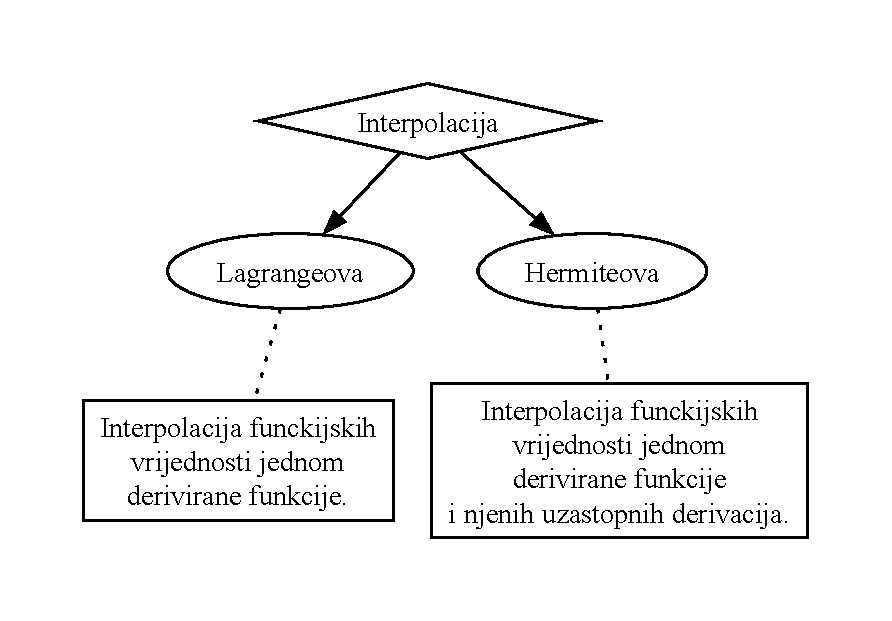
\includegraphics[width=0.5\linewidth]{interpolation.pdf}
\end{center}

\begin{theorembox}[egzistencija i jedinstvenost polinoma]
    Neka je $n\in\mathbb{N}_0$. Za zadane točke $(x_k,y_k)$, gdje je $y_k\coloneq f(x_k), k\in[0,n]$ i $x_i\neq x_j$ za $i\neq j$ postoji jedinstveni interpolacijski polinom najviše stupnja $n$

    $$
        p_n(x)=a_0+a_1x+\dots+a_nx^n
    $$

    za kojeg vrijedi

    $$
        p_n(x_k) = y_k,\qquad k\in[0,n]
    $$
\end{theorembox}

\textbf{Dokaz:}

\bigskip

Neka je polinom $p_n(x)=a_0+a_1x+a_2x^2+\dots+a_nx^n$ polinom stupnja najviše $n$.

Uvjete interpolacije zapisujemo u obliku

\begin{gather*}
    p_n(x_0)=a_0+a_1x_0+a_2x_0^2+\dots+a_nx_0^n=y_0\\
    p_n(x_1)=a_0+a_1x_1+a_2x_1^2+\dots+a_nx_1^n=y_1\\
    \vdots\\
    p_n(x_n)=a_0+a_1x_n+a_2x_n^2+\dots+a_nx_n^n=y_2
\end{gather*}

Dobiven je sustav od $n+1$ linearne jednadžbe s $n+1$ nepoznanicom (koeficijenti $a_i, i\in[0,n]$ su nepoznanice).

Pitamo se ima li navedeni sustav rješenje i je li ono \textbf{jedinstveno}.
Za to je dovoljno provjeriti je li odgovarajuća matrica sustava regularna.\footnote{Matrica sustava je regularna ako joj je determinanta različita od 0.}
Matrični sustav koji promatramo je

\begin{equation}
    \label{unique_poly}
    \begin{bmatrix}
        1&x_0&x_0^2&\cdots&x_0^n\\
        1&x_1&x_1^2&\cdots&x_1^n\\
        \vdots\vdots&\vdots&\vdots&\vdots\\
        1&x_n&x_n^2&\cdots&x_n^n\\
    \end{bmatrix}
    \cdot
    \begin{bmatrix}
        a_0\\
        a_1\\
        \vdots\\
        a_n
    \end{bmatrix}
    =
    \begin{bmatrix}
        y_0\\
        y_1\\
        \vdots\\
        y_n
    \end{bmatrix}
\end{equation}

Želimo odrediti $D_n$, gdje je

$$
D_n = \begin{vmatrix}
    1&x_0&x_0^2&\cdots&x_0^n\\
    1&x_1&x_1^2&\cdots&x_1^n\\
    \vdots&\vdots&\vdots&\vdots&\vdots\\
    1&x_n&x_n^2&\cdots&x_n^n\\
\end{vmatrix}
$$

\newpage

Vandermondeova determinanta $D_n$ je poznata.
Ako je $D_n \neq 0$, tada sustav \ref{unique_poly} ima jedinstveno rješenje.
Definiramo pomoćnu determinantu oblika

$$
V_n(x) = \begin{vmatrix}
    1&x_0&x_0^2&\cdots&x_0^n\\
    1&x_1&x_1^2&\cdots&x_1^n\\
    \vdots&\vdots&\vdots&\vdots&\vdots\\
    1&x&x^2&\cdots&x^n\\
\end{vmatrix},
\qquad V_n(x_n) = D_n
$$

Promatramo li $V_n(x)$ kao funkciju od $x$, razvojem po posljednjem retku uočavamo da je $V_n(x)$
polinom stupnja najviše $n$ u varijabli $x$, a vodeći koeficijent tog polinoma je determinanta $D_{n-1}$.
Zaista vrijedi

\begin{gather*}
V_n(x)=(-1)^{n+1}\cdot\begin{vmatrix}
    x_0&x_0^2&\cdots&x_0^n\\
    x_1&x_1^2&\cdots&x_1^n\\
    \vdots&\vdots&\vdots&\vdots\\
    x_{n-1}&x_{n-1}^2&\cdots&x_{n-1}^n\\
\end{vmatrix}\cdot1
+(-1)^{n+2}\cdot\begin{vmatrix}
    1&x_0^2&\cdots&x_0^n\\
    1&x_1^2&\cdots&x_1^n\\
    \vdots&\vdots&\vdots&\vdots\\
    1&x_{n-1}^2&\cdots&x_{n-1}^n\\
\end{vmatrix}\cdot x
+\cdots\\
+\underbrace{(-1)^{2n}\cdot\begin{vmatrix}
    1&x_0&\cdots&x_0^{n-1}\\
    1&x_1&\cdots&x_1^{n-1}\\
    \vdots&\vdots&\vdots&\vdots\\
    1&x_{n-1}&\cdots&x_{n-1}^{n-1}\\
\end{vmatrix}}_{D_{n-1}}\cdot x^n
\end{gather*}

Dakle, vodeći koeficijent (koeficijent uz $x^n$) je

\begin{equation}
\label{unique_poly_coeff}
D_{n-1} = (-1)^{2n}\cdot\begin{vmatrix}
    1&x_0&\cdots&x_0^{n-1}\\
    1&x_1&\cdots&x_1^{n-1}\\
    \vdots&\vdots&\vdots&\vdots\\
    1&x_{n-1}&\cdots&x_{n-1}^{n-1}\\
\end{vmatrix}=\begin{vmatrix}
    1&x_0&\cdots&x_0^{n-1}\\
    1&x_1&\cdots&x_1^{n-1}\\
    \vdots&\vdots&\vdots&\vdots\\
    1&x_{n-1}&\cdots&x_{n-1}^{n-1}\\
\end{vmatrix}.
\end{equation}

Primjetimo da, ako se u $V_n(x)$ redom uvrste $x_0,x_1,\dots,x_{n-1}$, vrijedit će

$$
V_n(x_0)=V_n(x_1)=\dots=V_n(x_{n-1})=0,
$$

što povlači da su $x_0,x_1,\dots,x_{n-1}$ nultočke polinoma $V_n(x)$ koji je polinom $n$-tog stupnja.
Da bi polinom $n$-tog stupnja bio potpuno definiran, trebaju biti poznate nultočke i njegov
vodeći koeficijent (\ref{unique_poly_coeff}). Dakle, traženi polinom je

$$
V_n(x) = D_{n-1}(x-x_0)(x-x_1)\dots(x-x_{n-1}).
$$

Ako uvrstimo $x_n$ u $V_n(x)$, dobivamo rekurzivnu formulu za $D_n$, odnosno

$$
D_n=V_n(x_n)=D_{n-1}(x_n-x_0)(x_n-x_1)\dots(x_n-x_{n-1}).
$$

Trivijalno vrijedi $D_0 = 1$ te lako dobivamo

$$
D_n = \prod_{0\leq j<i\leq n}(x_i-x_j).
$$

Budući da je $x_i\neq x_j$ za $i\neq j$, onda je $D_n\neq 0$, a vrijedi i obrat.
Dakle, matrica sustava je regularna (jer $D_n\neq 0$) i stoga postoji jedinstveno rješenje
$(a_0,a_1,\dots,a_n)$ što povlači da postoji jedinstveni interpolacijski polinom.

\section{Vandermondeova determinanta}

Za $n$ zadanih točaka ($x_k$, $y_k$) gdje je $y_k := f(x_k)$, $k$ predstavlja indeks točke ($k = 0, 1, \dots, n$), ako ni jedne dvije točke nemaju istu $x$ vrijednost postoji jedinstveni \textbf{interpolacijski polinom} najviše stupnja $n$:
\begin{equation}
    p_n(x)\coloneq \sum_{i=0}^na_ix^i= a_0 + a_1x + \dots a_nx^n
\end{equation}

Sustavi dobiveni uporabom vandermondeove determinante su nestabilni te se zbog toga najčešće koristi baza polinoma koja daje stabilnije rezultate.

\begin{example}[uporaba vandermondeove determinante]
    Zadane su sljedeće točke, odredi interpolacijski polinom uporabom vandermondeove determinante:

    \center
    \begin{tabular}{r|c|c|c}
        $x$&0&2&4\\
        \hline
        $y$&3&4&2
    \end{tabular}
\end{example}

\begin{multicols}{2}

Zadane su 3 točke pa očekujemo polinom maksimalno drugog stupnja:

$$
    p_2(x) = a_0 + a_1x + a_2x^2
$$

Uvrštavanjem točaka dobivamo:

\begin{gather*}
p_2(0) = a_0\cdot 1 + a_1\cdot 0 + a_2\cdot 0^2 = 3\\
p_2(2) = a_0\cdot 1 + a_1\cdot 2 + a_2\cdot 2^2 = 4\\
p_2(4) = a_0\cdot 1 + a_1\cdot 4 + a_2\cdot 4^2 = 2
\end{gather*}

\newcolumn

Što predstavljeno kao matrična jednadžba izgleda kao:

\begin{gather*}
\begin{bmatrix}
1 & 0 & 0 \\
1 & 2 & 4 \\
1 & 4 & 16
\end{bmatrix}
\cdot
\begin{bmatrix}
a_0 \\ a_1 \\ a_2
\end{bmatrix}
=
\begin{bmatrix}
3 \\ 4 \\ 2
\end{bmatrix} \\\\
A\cdot X = B \\
X = A^{-1} \cdot B
\end{gather*}

\end{multicols}

Zatim računamo \textbf{vandermondeovu determinantu}:

$$
D_n =
det(A) =
\begin{vmatrix}
1 & 0 & 0 \\
1 & 2 & 4 \\
1 & 4 & 16
\end{vmatrix}
= 1 \cdot
\begin{vmatrix}
2 & 4 \\
4 & 16
\end{vmatrix}
= 32 - 16 = 16 \neq 0
$$

\begin{multicols}{2}

Kako bismo odredili $A^{-1}$ trebamo provjeriti da je $det(A)\neq0$, u suprotnom inverzna matrica ne postoji. U ovom primjeru, inverzna matrica je:

\begin{gather*}
A^{-1} =
\begin{bmatrix}
1 & 0 & 0\\
-{\frac{3}{4}} & 1 & -{\frac{1}{4}}\\
{\frac{1}{8}} & -{\frac{1}{4}} & {\frac{1}{8}}
\end{bmatrix}\\
X = A^{-1}\cdot B =
\begin{bmatrix}
1 & 0 & 0\\
-\frac{3}{4} & 1 & -\frac{1}{4}\\
\frac{1}{8} & -\frac{1}{4} & \frac{1}{8}
\end{bmatrix}
\cdot
\begin{bmatrix}
3 \\ 4 \\ 2
\end{bmatrix}
=
\begin{bmatrix}
3 \\ \frac{5}{4} \\ -\frac{3}{8}
\end{bmatrix}
\end{gather*}

Rješavanjem sustava dobivamo $a_0=3$, $a_1=\frac{5}{4}$,\break$a_2=-\frac{3}{8}$,
kao i interpolaciju funkcije:
$$
p_2(x) = 3 + \frac{5x}{4} + -\frac{3x^2}{8}
$$

\newcolumn

\vspace*{0pt}

\begin{tikzpicture}
    \begin{axis}[
        xmin=-1,xmax=5,
        ymin=-1,ymax=6
    ]
        \addplot[plotlinefound] expression[samples=100]{3 + 5/4*x - 3/8*x^2} node[pos=0.8,anchor=south west]{$y=\sin{2x}+\frac{1}{2}$};
        \addplot[plotinterpolated] coordinates {(0,3)};
        \addplot[plotinterpolated] coordinates {(2,4)};
        \addplot[plotinterpolated] coordinates {(4,2)};
    \end{axis}
\end{tikzpicture}

\end{multicols}

\section{Lagrangeov interpolacijski polinom}

Formula za Lagrangeov interpolacijski polinom (${\mathbf L}_n$) je:

\begin{align}
    {\mathbf I}_i(x) &\coloneq \prod_{\substack{j=0\\j\neq i}}^{n} \frac{x-x_j}{x_i-x_j}\\
    {\mathbf L}_n(x) &\coloneq \sum_{i=0}^{n} y_i\mathbf{I}_i(x)
\end{align}

Lagrangeov interpolacijski polinom je bolji od korištenja vandermondeove determinante jer su sustavi dobiveni vandermondeovom determinantom nestabilni.
Također je i postupak brži jer ne zahtijeva računanje inverzne matrice koja u računalnoj primjeni zahtijeva mnogo međukoraka i instrukcija.

\begin{example}[uporaba lagrangeovog polinoma]
    Odredi interpolacijski polinom koristeći lagrangeove polinome ako su zadane sljedeće točke:

    \center
    \begin{tabular}{r|c|c|c}
        $x$&-3&4&3\\
        \hline
        $y$&-4&2&0\\
    \end{tabular}
\end{example}

Računamo $\mathrm{I}_0(x), \mathrm{I}_1(x),$ i $\mathrm{I}_2(x)$ za točke:

$$
\mathrm{I}_0(x) = \frac{x-x_1}{x_0-x_1} \cdot \frac{x-x_2}{x_0-x_2} = \frac{x-4}{-3-4} \cdot \frac{x-3}{-3-3} = \frac{(x-4)(x-3)}{-7\cdot-6} = \frac{x^2-7x+12}{42}
$$

\begin{warningbox}[nedostajući član]
    $$
    \frac{x-x_j}{x_0-x_j}=\frac{x-x_0}{x_0-x_0}=\frac{x-x_0}{0}
    $$
\end{warningbox}

\begin{align*}
\mathrm{I}_1(x) &= \frac{(x-x_0)(x-x_2)}{(x_1-x_0)(x_1-x_2)} = \frac{(x+3)(x-3)}{7\cdot1} = \frac{x^2-9}{7}\\\\
\mathrm{I}_2(x) &= \frac{(x-x_0)(x-x_1)}{(x_2-x_0)(x_2-x_1)} = \frac{(x+3)(x-4)}{6\cdot-1} = \frac{x^2-x-12}{-6}
\end{align*}

\begin{multicols}{2}

\vspace*{0pt}

Nakon uvrštavanja dobivamo polinom:
\begin{align*}
\mathrm{L}_2(x) &= y_0\mathrm{I}_0(x) + y_1\mathrm{I}_1(x) + y_2\mathrm{I}_2(x)\\
&= -4\cdot\frac{x^2-7x+12}{42} + 2\cdot\frac{x^2-9}{7} + 0\cdot\frac{x^2-x-12}{-6}\\
&= \frac{-2x^2+14x-24+6x^2-54}{21}\\
&= \frac{4x^2}{21} + \frac{2x\cdot\cancel{7}}{3\cdot\cancel{7}} - \frac{26\cdot\cancel{3}}{7\cdot\cancel{3}}\\
&\boxed{= {\frac{4}{21}}x^2 + {\frac{2}{3}}x - {\frac{26}{7}}}
\end{align*}

\vspace*{0pt}

\newcolumn

\vspace*{0pt}

\begin{tikzpicture}
    \begin{axis}[
        xmin=-4,xmax=4.5,
        ymin=-5,ymax=3,
        ]
        \addplot[plotlinefound] expression[samples=100]{4/21*x^2 + 2/3*x - 26/7}
          node[pos=0.5, anchor=north west] {$y=\sin(2x) + \frac{1}{2}$};
        \addplot[plotinterpolated] coordinates {(-3,-4)};
        \addplot[plotinterpolated] coordinates {(4,2)};
        \addplot[plotinterpolated] coordinates {(3,0)};
    \end{axis}
\end{tikzpicture}

\end{multicols}

\subsection{Nedostaci}

\begin{definition}
    Funkcija $g(x)$ je reda $\mathcal{O}(h(x))$ za $x \to x_0$, odnosno
    $$
    g(x) = \mathcal{O}(h(x)), x\to x_0
    $$
    ako postoje konstante $\sigma, C$ takve da
    $$
    |x-x_0| \leq \sigma \Rightarrow |g(x)| \leq C|h(x)|
    $$
\end{definition}

\subsubsection{Veliki broj aritmetičkih operacija}

Interpolacija lagrangeovim polinomom zahtijeva $\mathcal{O}(n^2)$ operacija kod prvog izvrednjavanja i $\mathcal{O}(n)$ operacija za svako sljedeće izvrednjavanje.

Kod računalne primjene brzina izračuna ovisi u broju primjena dobivenog polinoma jer se unaprijed izračunata vandermondeova determinanta za sustav može primijeniti više puta dok je u slučaju lagrangeovih polinoma potrebno koristiti pokazivače na članove polinoma ($\mathrm{I}_n$, koji su parcijalno ispunjene funkcije na gomili) što npr. za crtanje funkcije \textbf{može zahtijevati veći broj dereferenciranja s gomile}.

Taj problem je rješiv korištenjem biblioteka za simboličku matematiku, no to povećava veličinu distribuirane binarne datoteke, iako je taj kompromis generalno primjeren ako se biblioteka koristi za pojednostavljivanje više izraza tokom izvođenja programa ili se radi o jednonamjenskom programu.

\subsubsection{Velika zavisnost o ulaznim podacima}

U slučaju izmjena ulaznih podataka (ponajviše x koordinata) je potrebno ponovo računati sve polinome interpolacije ($\mathrm{I}_n$).

Kod računalne primjene, prethodno navedene parcijalno ispunjene funkcije (za $\mathrm{I}_n$) je potrebno ponovo slagati - \textbf{loša memoizacija}.

\subsubsection{Slaba aproksimacija i oscilacije}

Ako se odabere polinom preniskog stupnja, on može \textbf{slabo aproksimirati originalnu funkciju}.

\textbf{Rungeov fenomen}: Ako se odabere polinom previsokog stupnja, na dijelovima se mogu pojaviti \textbf{prevelike oscilacije}, tj. greške na rubovima intervala aproksimacije.


\section{Newtonov interpolacijski polinom}

Newtonov interpolacijski polinom rješava problem loše memoizacije koji lagrangeov polinom ima prilikom dodavanja interpoliranih točaka. Rješava to jer je definiran kao \textbf{rekurzivna funkcija} kojoj se \textbf{mogu pridodati članovi} kako bi aproksimacija davala točne vrijednosti za novonastali skup:

\begin{equation}
{\mathbf p}_n(x) \coloneq \mathbf{p}_{n-1}(x) + \mathbf{c}(x)
\end{equation}

${\mathbf c}(x)$ nazivamo korekcijom, i ona je polinom stupnja $n$, oblika:

\begin{equation}
{\mathbf c}(x) \coloneq {\mathbf a}_n\prod_{i=0}^{n-1}(x-x_i) = {\mathbf a}_n(x-x_0)(x-x_1)\dots(x-x_{n-1}).
\end{equation}

\subsection{Podijeljena razlika}

$\mathbf{a}_n$ je funkcija čvorova $x_i,\space i=0, 1, \dots, n$ koju zovemo \textbf{podijeljena razlika $n$-tog reda} i označavamo:

\begin{align*}
\mathbf{a}_n &\coloneq f[x_0,\dots,x_n]\\
\mathrm{a}_0 = f[x_0] &\coloneq f(x_0)
\end{align*}

Za \textit{dvije točke} ($x_0$,$f(x_0)$), ($x_1$,$f(x_1)$) definiramo i označavamo \textbf{podijeljenu razliku prvog reda funkcije} $f$ kao:

$$
f[x_0, x_1] = \frac{f(x_1)-f(x_0)}{x_1 - x_0} = \frac{f(x_0)}{x_0 - x_1} + \frac{f(x_1)}{x_1 - x_0}
$$

Za \textit{tri točke} ($x_0$,$f(x_0)$), ($x_1$,$f(x_1)$), ($x_2$,$f(x_2)$) uvodimo \textbf{podijeljenu razliku drugog reda funkcije} $f$ kao:

\begin{gather*}
    f[x_0, x_1, x_2] = \frac{f[x_2,x_1]-f[x_1,x_0]}{x_2 - x_0} = \frac{\displaystyle\frac{f(x_2)}{x_2 - x_1}-\frac{f(x_1)}{x_2 - x_1}}{x_2 - x_0}-\frac{\displaystyle\frac{f(x_1)}{x_1 - x_0}-\frac{f(x_0)}{x_1 - x_0}}{x_2 - x_0}\\\\
    = \frac{f(x_2)}{(x_2-x_0)(x_2-x_1)}-\frac{f(x_1)}{(x_2-x_0)(x_2-x_1)}-\frac{f(x_1)}{(x_2-x_0)(x_1-x_0)}+\frac{f(x_0)}{(x_2-x_0)(x_1-x_0)}\\
    = \frac{f(x_0)}{(x_2-x_0)(x_1-x_0)}-\frac{f(x_1)(x_1-x_0)+f(x_1)(x_2-x_1)}{(x_2-x_0)(x_1-x_0)(x_2-x_1)}+\frac{f(x_2)}{(x_2-x_0)(x_2-x_1)}\\
    = \frac{f(x_0)}{(x_2-x_0)(x_1-x_0)}-\frac{f(x_1)(\cancel{x_1}-x_0+x_2\cancel{-x_1})}{(x_2-x_0)(x_1-x_0)(x_2-x_1)}+\frac{f(x_2)}{(x_2-x_0)(x_2-x_1)}\\
    = \frac{f(x_0)}{(x_2-x_0)(x_1-x_0)}-\frac{f(x_1)\cancel{(x_2-x_0)}}{\cancel{(x_2-x_0)}(x_1-x_0)(x_2-x_1)}+\frac{f(x_2)}{(x_2-x_0)(x_2-x_1)}\\
    = \frac{f(x_0)}{(x_2-x_0)(x_1-x_0)}-\frac{f(x_1)}{(x_1-x_0)(x_2-x_1)}+\frac{f(x_2)}{(x_2-x_0)(x_2-x_1)}\\
    = \frac{f(x_0)}{(x_2-x_0)(x_1-x_0)}\cancel{-}\frac{f(x_1)}{(x_1-x_0)\cdot\cancel{-1}\cdot(x_1-x_2)}+\frac{f(x_2)}{(x_2-x_0)(x_2-x_1)}\\\\
    \boxed{
    = \frac{f(x_0)}{(x_0-x_1)(x_0-x_2)}+\frac{f(x_1)}{(x_1-x_0)(x_1-x_2)}+\frac{f(x_2)}{(x_2-x_0)(x_2-x_1)}
    }
\end{gather*}

\newpage

Zbog pojednostavljivanja rekurzivnog izračuna je poželjno zapisati podijeljene razlike u obliku tablice:

\begin{tablebox}[podijeljene razlike]
    $$
    \begin{array}{ccccccc}
        x_0 & f[x_0] \\
        & & f[x_0, x_1] \\
        x_1 & f[x_1] & & f[x_0, x_1, x_2] \\
        & & f[x_1, x_2] & & f[x_0, x_1, x_2, x_3] \\
        x_2 & f[x_2] & & f[x_1, x_2, x_3] & \vdots \\
        & & f[x_2, x_3] & \vdots & & \cdots & f[x_0, x_1, \dots, x_n] \\
        x_3 & f[x_3] & \vdots \\
        \vdots & \vdots & & f[x_{n-2}, x_{n-1}, x_n] \\
        & & f[x_{n-1}, x_n] \\
        x_n & f[x_n] \\
    \end{array}
    $$
\end{tablebox}

Općenita rekurzivna relacija koja vrijedi za podijeljene razlike je:

$$
f[x_0, x_1, \dots, x_n] = \frac{f[x_1, \dots, x_n]- f[x_0, \dots, x_{n-1}]}{x_n - x_0}
$$

Indukcijom iz rekurzivne relacije izvodimo \textbf{lineariziran oblik za podijeljenu razliku $n$-tog reda} koji nije rekurzivan:

$$
f[x_a, \dots, x_b] = \sum_{i=a}^{b} \frac{f(x_i)}{\prod_{\substack{j=a\\j\neq i}}^b(x_i - x_j)},\qquad a>0,\qquad b>a
$$

Taj oblik je praktičan za primjenu prilikom ručnog izračuna jer ne zahtijeva rekurzivno raspisivanje svih članova.

Iz toga također slijedi sažeti zapis newtonovog polinoma:

$$
p_n(x) = \sum_{i=1}^{n}\left[\left(\sum_{j=0}^{i} \frac{f(x_j)}{\prod_{\substack{k=0\\k\neq j}}^i(x_j - x_k)}\right)\prod_{j=0}^{i-1}(x-x_j)\right]
$$

Ovaj zapis je malo manje praktičan, no daje potpun uvid u polinom.

\begin{warningbox}[međupohrana]
    Direktan izračun gubi prednost međupohrane djelomičnih rezultata koji se mogu ponovo uporabiti prilikom dodavanja interpoliranih točaka.

    Kod računalnog izračuna ima smisla pohraniti rezultate podijeljenih razlika ($f[\dots]$) u međuspremnik te po potrebi izračunati vrijednost polinoma $p_n$ s njima.
\end{warningbox}

\newpage

\subsection{Ekvidistantni čvorovi}

U slučaju jednako udaljenih (ekvidistantnih) čvorova je podijeljena razlika jednostavnija za zapisati te se zove \textbf{konačna razlika}.

Ekvidistantne čvorove možemo zapisati u obliku:

$$
x_{i+1}=x_i+h,\qquad i\in[0,n\rangle
$$

gdje je $h$ konstantan razmak (korak) između dva susjedna čvora.

Konačna razlika je oblika:

\begin{align}
\label{kon_razl}
\Delta^kf(x_i) &\coloneq \Delta^{k-1}f(x_{i+1}) - \Delta^{k-1}f(x_i),\qquad k\in\langle0,n]\\\nonumber\\
\Delta^0f(x_i) &\coloneq f(x_i)\nonumber
\end{align}

\begin{tablebox}[konačne razlike]
    $$
    \begin{array}{ccccccc}
        x_0 & f(x_0) \\
        & & \Delta f(x_0) \\
        x_1 & f(x_1) & & \Delta^2 f(x_0) \\
        & & \Delta f(x_1) & & \Delta^3 f(x_0) \\
        x_2 & f(x_2) & & \Delta^2 f(x_1) & \vdots \\
        & & \Delta f(x_2) & \vdots & & \cdots & \Delta^n f(x_0) \\
        x_3 & f(x_3) & \vdots \\
        \vdots & \vdots & & \Delta^2 f(x_{n-2}) \\
        & & \Delta f(x_{n-1}) \\
        x_n & f(x_n) \\
    \end{array}
    $$
\end{tablebox}

Vrijedi \textbf{lema o vezi podijeljenih i konačnih razlika}:

$$
f[x_0,x_1,\dots,x_n] = \frac{\Delta^nf(x_0)}{n!h^n},\qquad x_{i+1}-x_i=h,\qquad i\in [0,n\rangle
$$

Zbog leme o vezi razlika, tablica konačnih razlika izgleda identično tablici podijeljenih razlika.

Newtonov oblik interpolacijskog polinoma na ekvidistantnim čvorovima je:

\begin{align}
p_n(x) =& \sum_{i=1}^{n}\left(\frac{\Delta^if(x_0)}{i!h^i}\prod_{j=0}^{i-1}x-x_j\right)\\\nonumber\\
=&f(x_0)
+\frac{\Delta f(x_0)}{1!h}(x-x_0)
+\frac{\Delta^2 f(x_0)}{2!h^2}(x-x_0)(x-x_1)
+\dots
+\frac{\Delta^n f(x_0)}{n!h^n}(x-x_0)\dots(x-x_{n-1})\nonumber
\end{align}

\newpage

\begin{example}
    Funkciju $f(x)=sin(\pi x)$ na segmentu [0, 1] aproksimirati interpolacijskim polinomom koji prolazi sljedećim točkama:

    \center
    \begin{tabular}{r|c|c|c|c|c}
        $x$ & 0 & 0.25 & 0.5 & 0.75 & 1\\
        \hline
        $f(x)$ & 0 & 0.7071 & 1 & 0.7071 & 0
    \end{tabular}
\end{example}

S obzirom na to da su zadane točke sve podjednako udaljene ($h=0.25$), možemo koristiti newtonovu interpolaciju za ekvidistantne točke:

\begin{align*}
p_4(x) =& f(x_0) + \frac{\Delta^1f(x_0)}{1!h^1}(x-x_0) + \frac{\Delta^2f(x_0)}{2!h^2}(x-x_0)(x-x_1)+\\
&\frac{\Delta^3f(x_0)}{3!h^3}(x-x_0)(x-x_1)(x-x_2)+\frac{\Delta^4f(x_0)}{4!h^4}(x-x_0)(x-x_1)(x-x_2)(x-x_3)
\end{align*}

Popunjavamo tablicu konačnih razlika prema formuli \ref{kon_razl}:

$$
\begin{array}{cccccc}
    0 & 0 \\
    & & \Delta f(x_0) = 0.7071 \\
    0.25 & 0.7071 & & \Delta^2 f(x_0) = -0.4142 \\
    & & \Delta f(x_1) = 0.2929 & & \Delta^3 f(x_0) = -0.1716 \\
    0.5 & 1 & & \Delta^2 f(x_1) = -0.5858 & & \Delta^4 f(x_0) = 0.3432 \\
    & & \Delta f(x_2) = -0.2929 & & \Delta^3 f(x_1) = 0.1716 \\
    0.75 & 0.7071 & & \Delta^2 f(x_1) = -0.4142 \\
    & & \Delta f(x_0) = -0.7071 \\
    1 & 0 \\
\end{array}
$$

Nakon što smo odredili sve konačne razlike, možemo ih uvrstiti u prethodnu formulu:

\begin{align*}
p_4(x) =&\, 0 + \frac{0.7071}{1!\cdot0.25^1}(x-0) + \frac{-0.4142}{2!\cdot0.25^2}(x-0)(x-0.25)
+\frac{-0.1716}{3!\cdot0.25^3}(x-0)(x-0.25)(x-0.5)\\
&+\frac{0.3432}{4!\cdot0.25^4}(x-0)(x-0.25)(x-0.5)(x-0.75)\\
=&\,2.8284x − 3.3136x(x − 0.25) − 1.8304x(x − 0.25)(x − 0.5) + 3.6608x(x − 0.25)(x − 0.5)(x − 0.75)\\
=&\,3.6608x^4 - 7.3216x^3 + 0.576x^2 + 3.0848x
\end{align*}

\begin{tikzpicture}
    \begin{axis}[
        domain=-3:4,
        ymin=-1.5,ymax=2,
        ]
        \addplot[plotlinefound] expression[domain=-1:2,samples=100]{3.6608*\x^4 - 7.3216*\x^3 + 0.576*\x^2 + 3.0848*\x} 
                    node[pos=0.325,anchor=south east]{$p_4(x)$};
        \addplot[plotlinetarget] expression[samples=100]{sin(deg(pi*\x))} 
                    node[pos=0.2,anchor=east]{$f(x)$};
        \addplot[plotinterpolated] coordinates {(0,0)};
        \addplot[plotinterpolated] coordinates {(0.25,0.7071)};
        \addplot[plotinterpolated] coordinates {(0.5,1)};
        \addplot[plotinterpolated] coordinates {(0.75,0.7071)};
        \addplot[plotinterpolated] coordinates {(1,0)};
    \end{axis}
\end{tikzpicture}

\newpage

\subsection{Računanje newtonovog polinoma u Pythonu}

\begin{example}
    Odredite vrijednost newtonovog polinoma točaka iz prethodnog zadatka u
    Pythunu za $x=1.5$.
\end{example}


\section{Newtonov interpolacijski polinom}

Newtonov interpolacijski polinom rješava problem loše memoizacije koji lagrangeov polinom ima prilikom dodavanja interpoliranih točaka. Rješava to jer je definiran kao \textbf{rekurzivna funkcija} kojoj se \textbf{mogu pridodati članovi} kako bi aproksimacija davala točne vrijednosti za novonastali skup:

\begin{equation}
{\mathbf p}_n(x) \coloneq \mathbf{p}_{n-1}(x) + \mathbf{c}(x)
\end{equation}

${\mathbf c}(x)$ nazivamo korekcijom, i ona je polinom stupnja $n$, oblika:

\begin{equation}
{\mathbf c}(x) \coloneq {\mathbf a}_n\prod_{i=0}^{n-1}(x-x_i) = {\mathbf a}_n(x-x_0)(x-x_1)\dots(x-x_{n-1}).
\end{equation}

\subsection{Podijeljena razlika}

$\mathbf{a}_n$ je funkcija čvorova $x_i,\space i=0, 1, \dots, n$ koju zovemo \textbf{podijeljena razlika $n$-tog reda} i označavamo:

\begin{align*}
\mathbf{a}_n &\coloneq f[x_0,\dots,x_n]\\
\mathrm{a}_0 = f[x_0] &\coloneq f(x_0)
\end{align*}

Za \textit{dvije točke} ($x_0$,$f(x_0)$), ($x_1$,$f(x_1)$) definiramo i označavamo \textbf{podijeljenu razliku prvog reda funkcije} $f$ kao:

$$
f[x_0, x_1] = \frac{f(x_1)-f(x_0)}{x_1 - x_0} = \frac{f(x_0)}{x_0 - x_1} + \frac{f(x_1)}{x_1 - x_0}
$$

Za \textit{tri točke} ($x_0$,$f(x_0)$), ($x_1$,$f(x_1)$), ($x_2$,$f(x_2)$) uvodimo \textbf{podijeljenu razliku drugog reda funkcije} $f$ kao:

\begin{gather*}
    f[x_0, x_1, x_2] = \frac{f[x_2,x_1]-f[x_1,x_0]}{x_2 - x_0} = \frac{\displaystyle\frac{f(x_2)}{x_2 - x_1}-\frac{f(x_1)}{x_2 - x_1}}{x_2 - x_0}-\frac{\displaystyle\frac{f(x_1)}{x_1 - x_0}-\frac{f(x_0)}{x_1 - x_0}}{x_2 - x_0}\\\\
    = \frac{f(x_2)}{(x_2-x_0)(x_2-x_1)}-\frac{f(x_1)}{(x_2-x_0)(x_2-x_1)}-\frac{f(x_1)}{(x_2-x_0)(x_1-x_0)}+\frac{f(x_0)}{(x_2-x_0)(x_1-x_0)}\\
    = \frac{f(x_0)}{(x_2-x_0)(x_1-x_0)}-\frac{f(x_1)(x_1-x_0)+f(x_1)(x_2-x_1)}{(x_2-x_0)(x_1-x_0)(x_2-x_1)}+\frac{f(x_2)}{(x_2-x_0)(x_2-x_1)}\\
    = \frac{f(x_0)}{(x_2-x_0)(x_1-x_0)}-\frac{f(x_1)(\cancel{x_1}-x_0+x_2\cancel{-x_1})}{(x_2-x_0)(x_1-x_0)(x_2-x_1)}+\frac{f(x_2)}{(x_2-x_0)(x_2-x_1)}\\
    = \frac{f(x_0)}{(x_2-x_0)(x_1-x_0)}-\frac{f(x_1)\cancel{(x_2-x_0)}}{\cancel{(x_2-x_0)}(x_1-x_0)(x_2-x_1)}+\frac{f(x_2)}{(x_2-x_0)(x_2-x_1)}\\
    = \frac{f(x_0)}{(x_2-x_0)(x_1-x_0)}-\frac{f(x_1)}{(x_1-x_0)(x_2-x_1)}+\frac{f(x_2)}{(x_2-x_0)(x_2-x_1)}\\
    = \frac{f(x_0)}{(x_2-x_0)(x_1-x_0)}\cancel{-}\frac{f(x_1)}{(x_1-x_0)\cdot\cancel{-1}\cdot(x_1-x_2)}+\frac{f(x_2)}{(x_2-x_0)(x_2-x_1)}\\\\
    \boxed{
    = \frac{f(x_0)}{(x_0-x_1)(x_0-x_2)}+\frac{f(x_1)}{(x_1-x_0)(x_1-x_2)}+\frac{f(x_2)}{(x_2-x_0)(x_2-x_1)}
    }
\end{gather*}

\newpage

Zbog pojednostavljivanja rekurzivnog izračuna je poželjno zapisati podijeljene razlike u obliku tablice:

\begin{tablebox}[podijeljene razlike]
    $$
    \begin{array}{ccccccc}
        x_0 & f[x_0] \\
        & & f[x_0, x_1] \\
        x_1 & f[x_1] & & f[x_0, x_1, x_2] \\
        & & f[x_1, x_2] & & f[x_0, x_1, x_2, x_3] \\
        x_2 & f[x_2] & & f[x_1, x_2, x_3] & \vdots \\
        & & f[x_2, x_3] & \vdots & & \cdots & f[x_0, x_1, \dots, x_n] \\
        x_3 & f[x_3] & \vdots \\
        \vdots & \vdots & & f[x_{n-2}, x_{n-1}, x_n] \\
        & & f[x_{n-1}, x_n] \\
        x_n & f[x_n] \\
    \end{array}
    $$
\end{tablebox}

Općenita rekurzivna relacija koja vrijedi za podijeljene razlike je:

$$
f[x_0, x_1, \dots, x_n] = \frac{f[x_1, \dots, x_n]- f[x_0, \dots, x_{n-1}]}{x_n - x_0}
$$

Indukcijom iz rekurzivne relacije izvodimo \textbf{lineariziran oblik za podijeljenu razliku $n$-tog reda} koji nije rekurzivan:

$$
f[x_a, \dots, x_b] = \sum_{i=a}^{b} \frac{f(x_i)}{\prod_{\substack{j=a\\j\neq i}}^b(x_i - x_j)},\qquad a>0,\qquad b>a
$$

Taj oblik je praktičan za primjenu prilikom ručnog izračuna jer ne zahtijeva rekurzivno raspisivanje svih članova.

Iz toga također slijedi sažeti zapis newtonovog polinoma:

$$
p_n(x) = \sum_{i=1}^{n}\left[\left(\sum_{j=0}^{i} \frac{f(x_j)}{\prod_{\substack{k=0\\k\neq j}}^i(x_j - x_k)}\right)\prod_{j=0}^{i-1}(x-x_j)\right]
$$

Ovaj zapis je malo manje praktičan, no daje potpun uvid u polinom.

\begin{warningbox}[međupohrana]
    Direktan izračun gubi prednost međupohrane djelomičnih rezultata koji se mogu ponovo uporabiti prilikom dodavanja interpoliranih točaka.

    Kod računalnog izračuna ima smisla pohraniti rezultate podijeljenih razlika ($f[\dots]$) u međuspremnik te po potrebi izračunati vrijednost polinoma $p_n$ s njima.
\end{warningbox}

\newpage

\subsection{Ekvidistantni čvorovi}

U slučaju jednako udaljenih (ekvidistantnih) čvorova je podijeljena razlika jednostavnija za zapisati te se zove \textbf{konačna razlika}.

Ekvidistantne čvorove možemo zapisati u obliku:

$$
x_{i+1}=x_i+h,\qquad i\in[0,n\rangle
$$

gdje je $h$ konstantan razmak (korak) između dva susjedna čvora.

Konačna razlika je oblika:

\begin{align}
\label{kon_razl}
\Delta^kf(x_i) &\coloneq \Delta^{k-1}f(x_{i+1}) - \Delta^{k-1}f(x_i),\qquad k\in\langle0,n]\\\nonumber\\
\Delta^0f(x_i) &\coloneq f(x_i)\nonumber
\end{align}

\begin{tablebox}[konačne razlike]
    $$
    \begin{array}{ccccccc}
        x_0 & f(x_0) \\
        & & \Delta f(x_0) \\
        x_1 & f(x_1) & & \Delta^2 f(x_0) \\
        & & \Delta f(x_1) & & \Delta^3 f(x_0) \\
        x_2 & f(x_2) & & \Delta^2 f(x_1) & \vdots \\
        & & \Delta f(x_2) & \vdots & & \cdots & \Delta^n f(x_0) \\
        x_3 & f(x_3) & \vdots \\
        \vdots & \vdots & & \Delta^2 f(x_{n-2}) \\
        & & \Delta f(x_{n-1}) \\
        x_n & f(x_n) \\
    \end{array}
    $$
\end{tablebox}

Vrijedi \textbf{lema o vezi podijeljenih i konačnih razlika}:

$$
f[x_0,x_1,\dots,x_n] = \frac{\Delta^nf(x_0)}{n!h^n},\qquad x_{i+1_-x}i=h,\qquad i\in [0,n\rangle
$$

Zbog leme o vezi razlika, tablica konačnih razlika izgleda identično tablici podijeljenih razlika.

Newtonov oblik interpolacijskog polinoma na ekvidistantnim čvorovima je:

\begin{align}
p_n(x) =& \sum_{i=1}^{n}\left(\frac{\Delta^if(x_0)}{i!h^i}\prod_{j=0}^{i-1}x-x_j\right)\\\nonumber\\
=&f(x_0)
+\frac{\Delta f(x_0)}{1!h}(x-x_0)
+\frac{\Delta^2 f(x_0)}{2!h^2}(x-x_0)(x-x_1)
+\dots
+\frac{\Delta^n f(x_0)}{n!h^n}(x-x_0)\dots(x-x_{n-1})\nonumber
\end{align}

\newpage

\begin{examplebox}
    Funkciju $f(x)=sin(\pi x)$ na segmentu [0, 1] aproksimirati interpolacijskim polinomom koji prolazi sljedećim točkama:

    \center
    \begin{tabular}{r|c|c|c|c|c}
        $x$ & 0 & 0.25 & 0.5 & 0.75 & 1\\
        \hline
        $f(x)$ & 0 & 0.7071 & 1 & 0.7071 & 0
    \end{tabular}
\end{examplebox}

S obzirom na to da su zadane točke sve podjednako udaljene ($h=0.25$), možemo koristiti newtonovu interpolaciju za ekvidistantne točke:

\begin{align*}
p_4(x) =& f(x_0) + \frac{\Delta^1f(x_0)}{1!h^1}(x-x_0) + \frac{\Delta^2f(x_0)}{2!h^2}(x-x_0)(x-x_1)+\\
&\frac{\Delta^3f(x_0)}{3!h^3}(x-x_0)(x-x_1)(x-x_2)+\frac{\Delta^4f(x_0)}{4!h^4}(x-x_0)(x-x_1)(x-x_2)(x-x_3)
\end{align*}

Popunjavamo tablicu konačnih razlika prema formuli \ref{kon_razl}:

$$
\begin{array}{cccccc}
    0 & 0 \\
    & & \Delta f(x_0) = 0.7071 \\
    0.25 & 0.7071 & & \Delta^2 f(x_0) = -0.4142 \\
    & & \Delta f(x_1) = 0.2929 & & \Delta^3 f(x_0) = -0.1716 \\
    0.5 & 1 & & \Delta^2 f(x_1) = -0.5858 & & \Delta^4 f(x_0) = 0.3432 \\
    & & \Delta f(x_2) = -0.2929 & & \Delta^3 f(x_1) = 0.1716 \\
    0.75 & 0.7071 & & \Delta^2 f(x_1) = -0.4142 \\
    & & \Delta f(x_0) = -0.7071 \\
    1 & 0 \\
\end{array}
$$

Nakon što smo odredili sve konačne razlike, možemo ih uvrstiti u prethodnu formulu:

\begin{align*}
p_4(x) =& 0 + \frac{0.7071}{1!\cdot0.25^1}(x-0) + \frac{-0.4142}{2!\cdot0.25^2}(x-0)(x-0.25)
+\frac{-0.1716}{3!\cdot0.25^3}(x-0)(x-0.25)(x-0.5)\\
&+\frac{0.3432}{4!\cdot0.25^4}(x-0)(x-0.25)(x-0.5)(x-0.75)\\
=&2.8284x − 3.3136x(x − 0.25) − 1.8304x(x − 0.25)(x − 0.5) + 3.6608x(x − 0.25)(x − 0.5)(x − 0.75)\\
=&3.6608x^4 - 7.3216x^3 + 0.576x^2 + 3.0848x
\end{align*}

\begin{tikzpicture}
    \begin{axis}[
        domain=-3:4,
        ymin=-1.5,ymax=2,
        ]
        \addplot[plotlinefound] expression[domain=-1:2,samples=100]{3.6608*\x^4 - 7.3216*\x^3 + 0.576*\x^2 + 3.0848*\x} 
                    node[pos=0.325,anchor=south east]{$p_4(x)$};
        \addplot[plotlinetarget] expression[samples=100]{sin(deg(pi*\x))} 
                    node[pos=0.2,anchor=east]{$f(x)$};
        \addplot[plotinterpolated] coordinates {(0,0)};
        \addplot[plotinterpolated] coordinates {(0.25,0.7071)};
        \addplot[plotinterpolated] coordinates {(0.5,1)};
        \addplot[plotinterpolated] coordinates {(0.75,0.7071)};
        \addplot[plotinterpolated] coordinates {(1,0)};
    \end{axis}
\end{tikzpicture}

\newpage

\subsection{Ocjena greške lagrangeovog i newtonovog interpolacijskog polinoma}

Pod pretpostavkom da za svaki $f(x)$ postoji $f^{(n+1)}(x)$, gdje je $x \in [x_0,x_n]$ za neki $n\in\mathbb{N}_0$, i da su čvorovi interpolacijskog polinoma $p_n(x)$ za funkciju $f(x)$. Tada za svaki $x\in[x_0,x_n]$ postoji $\xi\in[x_0,x_n]$ takav da vrijedi:

$$
e(x) = f(x) - p_n(x) = \frac{\omega(x)}{(n + 1)!}f^{(n+1)}(\xi)
$$

Ako postoji $\mathrm{M}_{n+1} = \max_{x\in[x_0,x_n]}\left|f^{(n+1)}(x)\right|$, tada je globalna ocjena greške:

$$
|e(x)| = |f(x) - p_n(x)| \leq \frac{|\omega(x)|}{(n+1)!}\mathrm{M}_{n+1}
$$

\begin{examplebox}
    Odrediti grešku newtonovog interpolacijskog polinoma iz prethodnog zadatka u točki $x=0.6$ te odrediti globalnu ocjenu greške funkcije na zadanom segmentu.
\end{examplebox}

Koristeći interpolacijski polinom iz prethodnog zadatka dobivamo $p_4(0.6) = 0.95121$ dok je $f(0.6) = 0.95105$. Uvrštavanjem u formulu za apsolutnu pogrešku dobivamo:

$$
|f(0.6)-p_4(0.6)| = 1.53483\cdot10^{-4}
$$

Prema teoremu o ocjeni lagrangeovog/newtonovog polinoma dobivamo:

\begin{gather}
|f(x)-p_4(x)| \leq \frac{\pi^5}{5!}|x(x-0.25)(x-0.5)(x-0.75)(x-1)|\\
\mathrm{M}_5=\max_{x\in[0,1]}(\sin(\pi x))^{(5)}
\end{gather}

Odnosno preciznije, jer vrijedi $\sin(\pi x)^{(5)} = \pi^5\cos(\pi x)$, $\mathrm{M}_5$ je:

$$
\mathrm{M}_5 = \max_{x\in[0,1]}\left|\pi^5\cos(\pi x)\right|
$$

Na intervalu $[0,1], \cos(\pi x)$ zauzima najveću vrijednost ($1$) za $x=0$ te time slijedi:

$$
\mathrm{M}_5 = \left|\pi^5\cos(\pi \cdot 0)\right| = \left|\pi^5\cdot1\right| = \pi^5
$$

\subsection{Nedostaci}

Newtonova interpolacija pati od istog nedostatka kao i lagrangeova gdje se s većim brojem interpoliranih točaka pojavljuju sve veče \textbf{oscilacija na rubovima interpoliranih točaka}.

Složenost newtonovog polinoma je ista lagrangeovom, no naknadne izmjene u praktičnoj primjeni zahtijevaju znatno manji broj ponovnih izračuna.


\subsection{Ocjena greške lagrangeovog i newtonovog interpolacijskog polinoma}

Pod pretpostavkom da za svaki $f(x)$ postoji $f^{(n+1)}(x)$, gdje je $x \in [x_0,x_n]$ za neki $n\in\mathbb{N}_0$, i da su čvorovi interpolacijskog polinoma $p_n(x)$ za funkciju $f(x)$. Tada za svaki $x\in[x_0,x_n]$ postoji $\xi\in[x_0,x_n]$ takav da vrijedi:

$$
e(x) = f(x) - p_n(x) = \frac{\omega(x)}{(n + 1)!}f^{(n+1)}(\xi)
$$

Ako postoji $\mathrm{M}_{n+1} = \max_{x\in[x_0,x_n]}\left|f^{(n+1)}(x)\right|$, tada je globalna ocjena greške:

$$
|e(x)| = |f(x) - p_n(x)| \leq \frac{|\omega(x)|}{(n+1)!}\mathrm{M}_{n+1}
$$

\begin{example}
    Odrediti grešku newtonovog interpolacijskog polinoma iz prethodnog zadatka u točki $x=0.6$ te odrediti globalnu ocjenu greške funkcije na zadanom segmentu.
\end{example}

Koristeći interpolacijski polinom iz prethodnog zadatka dobivamo $p_4(0.6) = 0.95121$ dok je $f(0.6) = 0.95105$. Uvrštavanjem u formulu za apsolutnu pogrešku dobivamo:

$$
|f(0.6)-p_4(0.6)| = 1.53483\cdot10^{-4}
$$

Prema teoremu o ocjeni lagrangeovog/newtonovog polinoma dobivamo:

\begin{gather}
|f(x)-p_4(x)| \leq \frac{\pi^5}{5!}|x(x-0.25)(x-0.5)(x-0.75)(x-1)|\\
\mathrm{M}_5=\max_{x\in[0,1]}(\sin(\pi x))^{(5)}
\end{gather}

Odnosno preciznije, jer vrijedi $\sin(\pi x)^{(5)} = \pi^5\cos(\pi x)$, $\mathrm{M}_5$ je:

$$
\mathrm{M}_5 = \max_{x\in[0,1]}\left|\pi^5\cos(\pi x)\right|
$$

Na intervalu $[0,1], \cos(\pi x)$ zauzima najveću vrijednost ($1$) za $x=0$ te time slijedi:

$$
\mathrm{M}_5 = \left|\pi^5\cos(\pi \cdot 0)\right| = \left|\pi^5\cdot1\right| = \pi^5
$$

\subsection{Određivanje greške newtonovog polinoma u Pythonu}

Taj izraz možemo zapisati u Pythonu kako bi dobili funkciju za računanje greške u nekoj točki $z$:

\input{../code/newton_err}

\subsection{Nedostaci}

Newtonova interpolacija pati od istog nedostatka kao i lagrangeova gdje se s većim brojem interpoliranih točaka pojavljuju sve veče \textbf{oscilacija na rubovima interpoliranih točaka}.

Složenost newtonovog polinoma je ista lagrangeovom, no naknadne izmjene u praktičnoj primjeni zahtijevaju znatno manji broj ponovnih izračuna.

\section{Linearni interpolacijski splajn}

Prilikom pokušaja interpolacije velikog broja točaka pojavljuje se problem sa oscilacijama na rubovima interpoliranih točaka gdje vrijedi:

$$
\lim_{n\to \infty}\max_{x\in[-1,1]}\left|f(x)-{\mathbf p}_n(x)\right| = +\infty
$$

Iz tog razloga se vrlo rijetko za interpolaciju koriste polinomi visokog stupnja ($>5$) jer ona ima loša svojstva.

Jedna od efikasnih metoda interpolacije je \textit{po dijelovima polinomna interpolacija} (engl. piecewise polynomial interpolation) gdje se na svim podsegmentima inicijalnog segmenta korise polinomi niskog stupnja:

$$
p_i \in \mathcal{P}_m
$$

gdje je $\mathcal{P}_m$ oznaka za \textbf{prsten polinoma} stupnja $m$.

Neka su zadani čvorovi interpolacije i \textbf{interpolicijski polinom dogovorenog i niskog stupnja} ($\phi$) na podsegmentima $[x_i,x_{i+1}]$ za $i\in[0,n\rangle$:

\begin{gather}
(x_i,y_i),\qquad i\in[0,n]\nonumber\\
\phi_{[x_i,x_{i+1}]} = p_i(x),\qquad i\in[0,n\rangle
\end{gather}

\begin{conditionbox}
    Iz uvijeta interpolacije $\phi(x_i) = y_i$ za $i\in[0,n]$:
    \begin{equation}
        \label{ls_continuation}
        p_{i-1}(x_i) = p_i(x_i)=y_i,\qquad i\in[1,n\rangle
    \end{equation}
    Dobivamo sljedećih $2n$ uvijeta kojima se osigurava neprekidnost funkcije $\phi(x)$:
    \begin{align}
        \label{ls_match_first}
        p_0(x_0) &= y_0\\
        \vdots\quad&\nonumber\\
        \label{ls_match_transition}
        p_{n-2}(x_{n-1}) &= p_{n-1}(x_n) = y_{n-1}\\
        \label{ls_match_last}
        p_{n-1}(x_n) &= y_n
    \end{align}
\end{conditionbox}

Uvijeti \ref{ls_continuation}, \ref{ls_match_first}, \ref{ls_match_transition} i \ref{ls_match_last} opisuju neprekidnost polinoma među interpoliranim podsegmentima.

Ako odaberemo da su polinomi $p_i(x)\in\mathcal{P}_1$ (polinomi prvog stupnja), tada imamo dovoljno uvjeta iz kojih možemo jedinstveno odrediti sve koeficijente linearnog interpolacijskog splajna.

\subsection{Linearni splajn}

Svakom podsegmentu $[x_i,x_{i+1}]$ pridužimo jedinstveni polinom $p_i(x)$ kojeg jednostavno zapisujemo u obliku lagrangeovog ili newtonovog interpolacijskog polinoma:

\begin{align*}
\text{Lagrangeov polinom:}\qquad p_i(x) =& \frac{x-x_{i+1}}{x_i-x_{i+1}}y_i + \frac{x-x_i}{x_{i+1}-x_i}y_{i+1}\\\\
\text{Newtonov polinom:}\qquad p_i(x) =& y_i + \frac{y_{i+1}-y_i}{x_{i+1}-x_i}(x-x_i)
\end{align*}

Linerani splajn se na kraju definira kao funkcija po dijelovima gdje je svaki dio definiran za pojedini segment kao pripadni polinom:

\begin{equation}
    \Phi(x)=\begin{cases}
        p_0(x),&x\in[x_0,x_1\rangle\\
        p_1(x),&x\in[x_1,x_2\rangle\\
        \quad\vdots&\\
        p_n(x),&x\in[x_n,x_{n+1}]\\
    \end{cases}
\end{equation}

\newpage

\begin{examplebox}[određivanje linearnog splajna]
    Odredi linearni splajn ako su zadane sljedeće točke:

    \center
    \begin{tabular}{r|c|c|c|c|c}
        x&0&1&2&3&4\\
        \hline
        y&0&0&1&1&0
    \end{tabular}
\end{examplebox}

\begin{multicols}{2}

Određujemo Newtonove interpolacijske polinome za sve tražene podsegmente:

\begin{align*}
    p_0(x)=y_0+\frac{y_1-y_0}{x_1-x_0}(x-x_0)&=0+\frac{0-0}{1-0}(x-0)=0\\
    p_1(x)=y_1+\frac{y_2-y_1}{x_2-x_1}(x-x_1)&=0+\frac{1-0}{2-1}(x-1)=x-1\\
    p_2(x)=y_2+\frac{y_3-y_2}{x_3-x_2}(x-x_2)&=1+\frac{1-1}{3-2}(x-2)=1\\
    p_3(x)=y_3+\frac{y_4-y_3}{x_4-x_3}(x-x_3)&=1+\frac{0-1}{4-3}(x-3)=4-x\\
\end{align*}

Te iz toga dobivamo formulu za linearni interpolacijski splajn:

$$
\Phi(x)=\begin{cases}
0,&x\in[0,1\rangle\\
x-1,&x\in[1,2\rangle\\
1,&x\in[2,3\rangle\\
4-x,&x\in[3,4]\\
\end{cases}
$$

\newcolumn

\begin{tikzpicture}
    \begin{axis}[
        domain=0:4,
        ymin=-1,ymax=2,
        ]
        \addplot[plotlinefound] expression[domain=0:1,samples=10]{0};
        \addplot[plotlinefound,color=cGreen] expression[domain=1:2,samples=10]{\x-1};
        \addplot[plotlinefound,color=cYellow] expression[domain=2:3,samples=10]{1};
        \addplot[plotlinefound,color=orange] expression[domain=3:4,samples=10]{4-\x};
        \addplot[plotinterpolated] coordinates {(0,0)};
        \addplot[plotinterpolated] coordinates {(1,0)};
        \addplot[plotinterpolated] coordinates {(2,1)};
        \addplot[plotinterpolated] coordinates {(3,1)};
        \addplot[plotinterpolated] coordinates {(4,0)};
    \end{axis}
\end{tikzpicture}

\end{multicols}

\subsection{Ocjena greške}

Ocjena greške linearnog splajna slijedi iz ovjene greške interpolacijskog polinoma.

Neka je $f(x)\in\mathcal{C}^2[a,b]$. Tada je ocjena greške interpolacije funkcije $f$ linearnim splajnom:

$$
|f(x)-\phi(x)| \leq \frac{\omega(x)\max_{x\in[x_i,x_{i+1}]}|f''(x)|}{2!}
$$

Uvođenjem oznaka $h=\max_{i\in[1,n]}|x_i-x_{i-1}|$ i $M=\max_{x\in[a,b]}|f''(x)|$ tada je $\omega(x)\leq{h^2\over4}$ pa za ocjenu greške linearnim splajnom vrijedi:

$$
|f(x) - \phi(x)|\leq \frac{\text{M}h^2}{8}
$$

Odnosno možemo pisati:

\begin{equation*}
    f(x) = \phi(x) + \mathcal{O}(h^2),\qquad h\to0
\end{equation*}

Kako bi se postigla zadovoljavajuća točnost ovom interpolacijom je potreban veliki broj podsegmenata, no zbog jednostavnosti se ipak vrlo često koristi kod računalne grafike.

Kada je potrebno približno odrediti vrijednost $f(\xi), \xi\in[a,b]$, prvo je potrebno odrediti u kojem se intervalu nalazi $\xi$. Da bi odredili $i$ takav da je $x_i\leq\xi\leq x_{i+1}$ najčešće se koristi binarno pretraživanje koje koristi $\mathcal{O}(\log(n))$ operacija.

$$
f(\xi)\approx p_i(\xi)
$$

\newpage

\begin{examplebox}[aproksimacija s točnošću]
    Aproksimirati funkciju $f(x) = \ln(x)$ na segmentu $[1,100]$ po dijelovima linearnom interpolacijom. Fiksirajmo traženu točnost $\varepsilon = 10^{-4}$ koju zahtijevamo na cijelom segmentu. Pronaći broj čvorova kako bi se postigla zadana točnost na:

    \begin{enumerate}
        \item ekvidistantnoj mreži s korakom $h$ na cijelom segmentu $[1,100]$
        \item podijeljenim podsegmentima $[1,2]$, $[2,7]$, $[7,100]$ gdje svaki od navedenih podsegmenata dijelimo ekvidistantnom mrežom čvorova s koracima $h_1$, $h_2$, $h_3$, respektivno.
    \end{enumerate}
\end{examplebox}

\textbf{1)} Određujemo:
    $$
    f'(x) = {1\over x},\qquad f''(x)={1\over x^2}\text{, te}\qquad |f''(x)|=\left|{1\over x^2}\right|={1\over x^2}.
    $$
    Promatrana funkcija uvijek postiže svoj maksimum u lijevom kraju segmenta $[1,100]$.

Koristeći ocjenu greške za linearni splajn, dobivamo da je na segmentu $[1, 100]$
uz ekvidistantnu mrežu s korakom $h$ greška interpolacije

$$
|\Phi(x)-f(x)|\leq\frac{1\cdot h^2}{8}.
$$

U našem slučaju mora vrijediti $\displaystyle\frac{h^2}{8}\leq 10^{-4}$ što povlači $h\leq0.02828$.
S obzirom na to da je

$$
h=\frac{b-a}{n}=\frac{100-1}{n}=\frac{99}{n},
$$

dobivamo da je $n=3500.17$, a budući da je $n\in\mathbb{N}$, tada u formulu nije uključen posljednji rubni čvor, zaključujemo da nam je za zadanu točnost potrebno barem $3501+1=3502$ čvorova.

\bigskip

\textbf{2)} Na svakom zadanom podsegmentu greška interpolacije mora biti manja od $\varepsilon=10^{-4}$.

\begin{itemize}
    \item Za prvi podsegment $[1,2]$ vrijedi $\text{M}_2(f) = 1$ pa je $\frac{h_1^2}{8}\leq10^{-4}$ što povlači $h_1\leq0.02828$, a analognim postupkom kao u prethodnom slučaju dobivamo da je $n_1\geq35.35$, odnosno $n_1=36$.
    \item Na drugom podsegmentu $[2,7]$ vrijedi $\text{M}_2(f) = {1\over4}$ pa je ${1\over4}\cdot\frac{h_2^2}{8}\leq10^{-4}$ odnosno $h_2\leq0.05656$ pa je $n_2\geq88.38$, odnosno $n_2=89$.
    \item Na trećem podsegmentu $[7,100]$ vrijedi $\text{M}_2(f) = {1\over49}$ pa je ${1\over49}\cdot\frac{h_3^2}{8}\leq10^{-4}$ odnosno $h_3\leq0.19798$ pa je $n_3\geq469.73$, odnosno $n_3=470$.
\end{itemize}

\subsection{Nedostaci}

Dok je aproksimacija danih podataka linearnim splajnom može biti dovoljna u nekim slučajevima, prijelazi između segmenata mogu biti pre nagli i primjetni za druge primjene. Na primjer:

\begin{itemize}
    \item brzina kretanja tijela u prostoru se može doimati \textit{neprirodnom},
    \item razlike u brzini porasta/pada amplitude zvuka su osjetne, \dots
\end{itemize}


\section{Kubični interpolacijski splajn}

Kako bi se izbjegao navedeni problem s tranzicijom između segmenata, poželjno je konstruirati splajn višeg reda.
\textbf{Kvadratni splajn} može imati skokove prve derivacije u točkama mreže čvorova pa se on ne primjenjuje toliko često.
\textbf{Kubični splajn} se iznimno često koristi u praksi te nema nedostatke koje imaju linearni i kvadratni splajn.

Kada imamo zadane diskretne vrijednosti funkcije:

\begin{equation*}
y_i=f(x_i),\qquad i\in[0,n]
\end{equation*}

i čvorove zadane tako da vrijedi:

$$
a\leq x_0 < x_1 < \dots < x_n \leq b
$$

Kubični splajn je funkcija $s(x)\in\mathcal{C}^2(\langle x_0,x_n\rangle)$ koja je:

\begin{itemize}
    \item na svakom podintervalu $[x_i, x_{i+1}\rangle, i\in[0,n\rangle$ polinom najviše trećeg stupnja,
    \item u čvorovima interpolacije zadovoljava uvjete interpolacije te
    \item ima neprekidnu drugu derivaciju
\end{itemize}

Na svakom podintervalu koriste se polinomi:

\begin{equation*}
\phi[x_i,x_{i+1}] = p_i(x),\qquad i\in[0,n],\qquad p_i(x)\in\mathcal{P}_3
\end{equation*}

Kubični polinom $p_i(x)$ ima četiri koeficijenta, i može se zapisati u obliku:

$$
p_i(x)=a_0+a_1(x-x_i)+a_2(x-x_i)^2+a_3(x-x_i)^3
$$

\begin{conditionbox}[određivanje koeficijenata kubičnog splajna]
    \begin{align}
        p_0(x_0) =& y_0\nonumber\\
        \label{cs_continuation}
        p_{i-1}(x_i) = p_i(x_i) =& y_i,\qquad i\in[1,n-1]\\
        p_{n-1}(x_n) =& y_n\nonumber\\\nonumber\\
        \label{cs_continuation_fd}
        p'_{i}(x_{i+1}) = p'_{i+1}(x_{i+1}) =& y_i,\qquad i\in[0,n-2]\\
        \label{cs_continuation_sd}
        p''_{i}(x_{i+1}) = p''_{i+1}(x_{i+1}) =& y_i,\qquad i\in[0,n-2]\\\nonumber\\
        s_0=&f'(x_0)\nonumber\\
        \label{cs_slope}
        s_n=&f'(x_n)
    \end{align}

    \begin{itemize}
        \item Uvjet \ref{cs_continuation} osigurava neprekidnost interpolacije i daje $2n$ uvjeta.
        \item Uvjet \ref{cs_continuation_fd} osigurava neprekidnost prve derivacije na unutarnjim čvorovima interpolacije i daje $n-1$ uvjeta.
        \item Uvjet \ref{cs_continuation_sd} osigurava neprekidnost druge derivacije na unutarnjim čvorovima interpolacije i daje dodatnih $n-1$ uvjeta.
        \item Uvjet \ref{cs_slope} osigurava da je nagib interpolacije na rubovima segmenata jednak nagibu funkcije.
    \end{itemize}

    \ref{cs_slope} je jedan on različitih načina za zadati dodatne uvijete kako bi dobili jedinstvena rješenja kubičnog splajna, tj. moguće je postići jedinstvenost rješenja i na druge načine.
\end{conditionbox}

\newpage

Označimo derivacije u unutarnjim čvorovima

\begin{equation*}
s_i=\phi'(x_i),\qquad i\in[1,n-1]
\end{equation*}

Polinome $p_i(x)$ u ovom slučaju je najpraktičnije zapisati u Newtonovom obliku interpolacijskog polinoma

$$
\begin{array}{ccccc}
    x_i & f[x_i]\\
    & & s_i\\
    x_i&f[x_i] & & f[x_i,x_i,x_{i+1}]\\
    & & f[x_{i+1},x_i] & & f[x_i,x_i,x_{i+1},x_{i+1}]\\
    x_{i+1} & f[x_{i+1}] & & f[x_i,x_{i+1},x_{i+1}]\\
    & & s_i\\
    x_{i+1} & f[x_{i+1}]\\
\end{array}
$$

Gdje su $s_i=f'(x_i)=f[x_i,x_i]$, a $s_{i+1}=f'(x_{i+1})=f[x_{i+1},x_{i+1}]$.

Iz definicije Newtonovog polinoma slijedi:

\begin{gather*}
p_i(x) = f[x_i]+f[x_i,x_i](x-x_i) + f[x_i,x_i,x_{i+1}](x-x_i)^2\\
+f[x_i,x_i,x_{i+1},x_{i+1}](x-x_i)^2(x-x_{i+1})
\end{gather*}

Isti polinom se može zapisati i u bazi $(x-x_i)^k$ kao:

$$
p_i(x)=\sum_{k=0}^3a_k(x-x_i)^k
$$

\begin{align*}
a_0=&f[x_i]&\qquad a_1=&s_i\\\\
a_2=&\frac{f[x_i,x_{i+1}]-s_i}{h_i}&\qquad a_3=&\frac{s_{i+1}+s_i-2f[x_i,x_{i+1}]}{h_i^2}
\end{align*}

pri čemu je $h_i=x_{i+1}-x_i$.

Iz uvjeta \ref{cs_continuation}-\ref{cs_slope} proizlazi sustav:

$$
h_is_{i-1}+2(h_{i-1}+h_i)s_i+h_{i-1}s_{i+1}=3(h_if[x_{i-1},x_i]+h_{i-1}f[x_i,x_{i+1}]),\qquad i\in[1,n-1]
$$

Dobiveni sustav je sastavljen od $n-1$ jednadžbi s $n-1$ nepoznanica i strogo je dijagonalno dominantan po redcima pa zaključujemo da je determinanta sustava različita od 0, odnosno sustav ima jedinstveno rješenje $\{s_1,\dots,s_{n-1}\}$ čime je potpuno određen kubični splajn.

\subsection{Druga derivacija na rubu segmenta}

\begin{conditionbox}[druga derivacija ruba]
    Kao što je prethodno navedeno uvjet \ref{cs_slope} nije jedini način za postizanje jedinstvenih rješenja. Možemo ih postići i s:
    \begin{align}
        \phi''_0=&f''(x_0)\nonumber\\
        \label{cs_sd}
        \phi''_n=&f''(x_n)
    \end{align}
    Ovdje uvjet \ref{cs_sd} osigurava da je stopa promjene nagiba ("savijenost") na rubovima interpoliranih segmenata jednaka nagibu funkcije.
\end{conditionbox}

Uvjeti \ref{cs_continuation}, \ref{cs_continuation_fd}, \ref{cs_continuation_sd} i \ref{cs_sd} dovode do linearnog sustava od $n+1$ jednadžbe s $n+1$ nepoznanicom, odnosno

\begin{align*}
p''_1(x_0) =& f''(x_0)\\
h_is_{i-1}+2(h_{i-1}+h_i)s_i+h_{i-1}s_{i+1}=&3(h_if[x_{i-1},x_i]+h_{i-1}f[x_i,x_{i+1}])\\
p''_n(x_n) =& f''(x_n)
\end{align*}

Dobiveni sustav je dijagonalno dominantan po redcima pa postoji jedinstveno rješenje sustava $\{s_0,\dots,s_n\}$. Funkcija $\phi(x)$ je klase $\mathcal{C}^2[a,b]$. Ako funkcija $f(x)$ ima omeđenu četvrtu derivaciju, tada vrijedi

$$
f(x)=\phi(x) + \mathcal(O)(h^4),\qquad h\to0.
$$

\newpage

\begin{example}[uporaba kubičnog splajna]
    Primjenom kubičnog splajna odrediti $\phi(2.33)$ i $\phi(4.21)$ ako su zadani podaci:
    
    \center
    \begin{tabular}{r|c|c|c|c|c}
        $x$ & 1 & 2 & 3 & 4 & 5 \\
        \hline
        $f(x)$ & 1 & 0.5 & 0.333 & 0.25 & 0.2 \\
        \hline
        $f'(x)$ & -0.5 & -0.25 & -0.111 & -0.0625 & -0.04
    \end{tabular}
\end{example}

U zadanoj tablici vrijedi $s_i=f'(x_i)$. Traženi polinomi su oblika $p_i(x)=\sum_{k=0}^3a_k(x-x_i)^k$ pa prema sljedećem određujemo vrijednosti koeficijenata $a_0$, $a_1$, $a_2$, $a_3$ za svaki podsegment posebno.

Tablica podijeljenih razlika je

$$
\begin{array}{ccc}
1&1&\\
&&-0.5\\
2&0.5\\
&&-0.167\\
3&0.333\\
&&-0.083\\
4&0.25\\
&&0.05\\
5&0.2\\
\end{array}
$$

\begin{multicols}{2}
\begin{itemize}
\item Za $p_1(x)$ na intervalu $[1,2\rangle$ vrijedi:
    \begin{gather*}
    a_0=f(x_0)=1,\qquad a_1=s_0=-0.5,\\
    a_2=\frac{f[x_0,x_1]-s_0}{h}-h\cdot a_3=-0.25,\\
    a_3=\frac{s_0+s_1-2f[x_0,x_1]}{h^2}=0.25,\\
    p_1(x)=1-0.5(x-1)-0.25(x-1)^2\\+0.25(x-1)^3
    \end{gather*}
\item Za $p_2(x)$ na intervalu $[2,3\rangle$ vrijedi:
    \begin{gather*}
    a_0=f(x_1)=0.5,\qquad a_1=s_1=-0.25,\\
    a_2=\frac{f[x_1,x_2]-s_1}{h}-h\cdot a_3=0.11,\\
    a_3=\frac{s_1+s_2-2f[x_1,x_2]}{h^2}=-0.027,\\
    p_2(x)=0.5-0.25(x-2)-0.027(x-2)^2\\+0.11(x-2)^3
    \end{gather*}
\newcolumn
\item Za $p_3(x)$ na intervalu $[3,4\rangle$ vrijedi:
    \begin{gather*}
    a_0=f(x_2)=1,\qquad a_1=s_2=-0.111,\\
    a_2=\frac{f[x_2,x_3]-s_2}{h}-h\cdot a_3=0.0355,\\
    a_3=\frac{s_2+s_3-2f[x_2,x_3]}{h^2}=-0.0075,\\
    p_3(x)=0.333-0.111(x-3)+0.0355(x-3)^2\\-0.0075(x-3)^3
    \end{gather*}
\item Za $p_4(x)$ na intervalu $[4,5\rangle$ vrijedi:
    \begin{gather*}
    a_0=f(x_3)=0.25,\qquad a_1=s_3=-0.0625,\\
    a_2=\frac{f[x_3,x_4]-s_3}{h}-h\cdot a_3=0.0015,\\
    a_3=\frac{s_3+s_4-2f[x_3,x_4]}{h^2}=-0.0025,\\
    p_4(x)=0.25-0.0625(x-4)+0.0015(x-4)^2\\-0.0025(x-4)^3
    \end{gather*}
\end{itemize}
\end{multicols}

Konačno, $\Phi(2.33)=p_2(2.33)=0.4286$.

\begin{tikzpicture}
    \begin{axis}[
        domain=1:5,
        ymin=-1,ymax=1,
        ]
        \addplot[plotlinefound] expression[domain=1:2,samples=10]{1-0.5*(\x-1)-0.25*(\x-1)^2+0.25*(\x-1)^3} node[pos=0.5,anchor=south]{$p_0$};
        \addplot[plotlinefound,color=cGreen] expression[domain=2:3,samples=10]{0.5-0.25*(\x-2)-0.027*(\x-2)^2+0.11*(\x-2)^3} node[pos=0.5,anchor=south]{$p_1$};
        \addplot[plotlinefound,color=cYellow] expression[domain=3:4,samples=10]{0.333-0.111*(\x-3)+0.0355*(\x-3)^2-0.0075*(\x-3)^3} node[pos=0.5,anchor=south]{$p_2$};
        \addplot[plotlinefound,color=orange] expression[domain=4:5,samples=10]{0.25-0.0625*(\x-4)+0.0015*(\x-4)^2-0.0025*(\x-4)^3} node[pos=0.5,anchor=south]{$p_3$};
        \addplot[plotinterpolated] coordinates {(1,1)};
        \addplot[plotinterpolated] coordinates {(2,0.5)};
        \addplot[plotinterpolated] coordinates {(3,0.333)};
        \addplot[plotinterpolated] coordinates {(4,0.25)};
        \addplot[plotinterpolated] coordinates {(5,0.2)};
    \end{axis}
\end{tikzpicture}

\newpage

\subsection{Greška kubičnog splajna}

Za kubični splajn ocjena greške je

\begin{align}
|f(x)-\phi(x)|\leq&\frac{\text{M}_4}{4!}\frac{h^4}{16}={1\over384}h^4\text{M}_4,\\
\text{M}_4=&\max_{x\in[a,b]}|f^{(IV)}(x)|,\\
h=&\max_{i\in[1,n]}h_i,\qquad h_i=x_{i+1}-x_i.
\end{align}

Drugim rjećima, ravnomjernim povećavanjem čvorova kubičnog splajna tako da $h\to0$, maksimalna greška te interpolacije se približava 0.


\section{Regresija}

Ni polinomijalna interpolacija ni kubični splajn nisu dobri za aproksimaciju vrijednosti koje nisu omeđene poznatim vrijednostima.
\begin{itemize}
    \item Kubični splajn ima manje oscilacije, no i dalje se pojavljuju značajne oscilacije i odstupanja na krajnjim segmentima.
    \item Interpolacijom se greške u mjerenim podacima "ugrađuju" u interpolacijsku funkciju.
\end{itemize}

Regresija je metoda određivanja funkcije koja blisko prati zadane podatke na način gdje opisuje njihovo ponašanje uz \textbf{minimalno rasipanje izmjerenih vrijednosti oko poznatih segmenata}. Dakle, neće davati vrijednosti jednake izmjerenim podacima, nego njima \textbf{bliske vrijednosti}.

\textbf{Udaljenost} $d_i$ zadane točke $(x_i, y_i)$ od točke na grafu se mjeri normom.
Najčešći izbor je $\mathrm{L}_2$ norma oblika

$$
d_i=\sqrt{(x_i-x_i)^2+(y_i-f(x_i))^2}.
$$

Tako se kao "najbliža" funkcija smatra onom kod koje su te udaljenosti po svim točkama najmanje. Budući da su $d_i\geq0, i\in[0,n]$, to znači da je \textbf{najbliža funkcija} ona kod koje je suma $\sum_{i=0}^nd_i$ najmanja.
Traženje minimuma te sume može biti problematično pa se u praksi uvijek traži minimum sume

\begin{equation}
    \label{sum_squares}
    \sum_{i=0}^nd_i^2
\end{equation}

koja daje jednake rezultate, ali ih je znatno lakše odrediti.

Minimiziranje sume kvadrata udaljenosti se smatra kriterijem kod metode regresije pa se metoda regresije također naziva i \textbf{metodom najmanjih kvadrata}.

Nemoguće je naći minimum sume \ref{sum_squares} na skupu svih mogućih funkcija. Za zadane točke \textbf{prvo biramo model ili klasu funkcije} između kojih ćemo tražiti onu koja minimizira sumu \ref{sum_squares}.

\subsection{Linearna regresija}

Najjednostavniji odabir je traženje funkcije na skupu svih pravaca $f(x) = a_0 + a_1x$ i takvu regresiju zovemo \textbf{linearna regresija}. Tako problem minimizacije \ref{sum_squares} svodimo na problem određivanja koeficijenata $a_0$ i $a_1$ u sumi

$$
S = \sum_{i=0}^n(y_i - (a_0+a_1x_i))^2
$$

Dakle radi se o funkciji $S=S(a_0,a_1)$ s dvije varijable kojoj jednostavno nalazimo minimum.

Prirodno, zadajemo uvjete za stacionarnu točku funkcije dvije varijable

$$
\partial_{a_0}S=0,\qquad\partial_{a_1}S=0.
$$

Nakon sređivanja uvjeti daju sustav dvije linearne jednadžbe

\begin{align*}
a_0(n+1)+a_1\sum_{i=0}^nx_i=&\sum_{i=0}^ny_i\\
a_0\sum_{i=0}^nx_i+a_1\sum_{i=0}^nx_i^2=&\sum_{i=0}^nx_iy_i
\end{align*}

za dvije nepoznanice $a_0$ i $a_1$.

Osim kod izuzetno nepovoljnog rasporeda točaka koji uistinu ne odgovara pravcu, ovaj \textbf{sustav ima determinantu različitu od nule} te time i jedinstveno rješenje, kada je broj točaka za koje ga rješavamo n$\geq2$.
Budući da je $S\geq0$, rješenje mora biti lokalni minimum te je time problem metode linearne regresije u potpunosti riješen.

\begin{example}[uporaba metode najmanjih kvadrata]
    Podatke zadane tablicom aproksimirati linearnom funkcijom koristeći metodu najmanjih kvadrata.

    \center
    \begin{tabular}{r|c|c|c}
        $x$ & 0 & 1 & 3 \\
        \hline
        $y$ & 1 & 2 & 3
    \end{tabular}
\end{example}

\subsection{Kvadratna regresija}

U slučaju kvadratne funkcije oblika

$$
f(x) = a_0+a_1x+a_2x^2
$$

imamo sumu

$$
S = \sum_{i=0}^n(y_i - (a_0+a_1x+a_2x^2))^2
$$

te potrebno zadati uvjete stacionarne točke za funkciju s 3 varijable:

$$
\partial_{a_0}S=0,\qquad\partial_{a_1}S=0,\qquad\partial_{a_2}S=0.
$$

Sređivanjem dobivamo sustav koji određuje koeficijente funkcije:

\begin{align*}
    a_0(n+1)+a_1\sum_{i=0}^nx_i+a_2\sum_{i=0}^nx_i^2=&\sum_{i=0}^ny_i,\\
    a_0\sum_{i=0}^nx_i+a_1\sum_{i=0}^nx_i^2+a_2\sum_{i=0}^nx_i^3=&\sum_{i=0}^nx_iy_i,\\
    a_0\sum_{i=0}^nx_i^2+a_1\sum_{i=0}^nx_i^3+a_2\sum_{i=0}^nx_i^4=&\sum_{i=0}^nx_i^2y_i.\\
\end{align*}

Budući da se određivanje nepoznatih koeficijenata svodi na rješavanje linearnog sustava, aproksimacija podataka kvadratnom funkcijom u smislu metode najmanjih kvadrata je opet linearan problem kada je broj točaka $n\geq3$.

\begin{example}
    Podatke zadane tablicom aproksimirati kvadratnom funkcijom koristeći metodu najmanjih kvadrata.

    \center
    \begin{tabular}{r|c|c|c|c|c}
        $x$ & -1 & -0.5 & 0.0 & 0.5 & 1.0 \\
        \hline
        $y$ & 1.0 & 0.5 & 0.0 & 0.5 & 0.2 \\
    \end{tabular}
\end{example}

\newpage

\subsection{Polinomna regresija}

I prethodnih regresija je vidljivo da je regresiju također moguće primijeniti u generalnom obliku koji je primjenjiv na sve polinomne funkcije stupnja $m$.

Regresija kojom se traži "najbliža" funkcija na skupu svih polinoma odabranog stupnja $m$:

$$
f(x) = a_0+a_1x+\dots+a_mx^m
$$

se zove \textbf{polinomna regresija polinomom stupnja} $\mathbf m$. Tako se nepoznavanje funkcije svodi na nepoznavanje $m+1$ koeficijenata $a_j, j\in[0,m]$.

Suma dobiva oblik

$$
S=\sum_{i=0}^n\left(y_i-\sum_{j=0}^ma_jx_i^j\right).
$$

Analogni polinomima nižeg stupnja, počinje se s uvjetom za stacionarnu točku funkcije više varijabli:

$$
\partial_{a_j}S=0,\qquad j\in[0,m].
$$

Nakon sređivanja jednadžbe poprimaju oblik:

$$
\sum_{k=0}^ma_k\sum_{i=0}^nx_i^{k+j}=\sum_{i=0}^nx_i^jy_i,\qquad j\in[0,m]
$$

Osim u slučajevima kad je polinomni model loš izbor za zadane točke, ovaj će sustav imati jedinstveno rješenje ako vrijedi $n\geq m$.

\subsection{Modeli svedeni na linearne}

Ostali modeli funkcija za zadane točke u pravilu će voditi na složenije probleme traženja minimuma sume po parametrima odabranog modela funkcije. Poželjno je izbjeći aproksimaciju polinomima višeg stupnja.

Neki od modela koje se može svesti na linearne su:

\begin{itemize}
    \item eksponencijalni model $y=ae^{bx}$ kojeg se svodi na linearni model $\ln y = \ln a+bx$ za točke $(x_i,\ln y_i), i\in[0,n]$,
    \item model potencije $y=ax^b$ kojeg se svodi na linearni model $\ln y = \ln a+b\ln x$ za točke $(\ln x_i, \ln y_i), i\in[0,n]$,
    \item model rasta do zasićenja $y=\frac{ab}{x+b}$ kojeg se svodi na linearni model ${1\over y}={1\over a}+{b\over ax}$ za točke $({1\over x_i}, {1\over y_i}), i\in[0,n]$.
\end{itemize}


\chapter{Određivanje nultočaka}

Cilj numeričkih metoda za rješavanje nelinearnih jednadžbi je odrediti
\textbf{nultočku (korijen, rješenje)} neprekidne ralne funkcije $f$ na segmentu
$[a,b]$, odnosno rješiti
$$
    f(x) = 0\,.
$$

Moguće je da
\begin{itemize}
    \item funkcija $f$ ima više realnih nultočaka i da su neke višestruke, kao i
    da
    \item funkcija $f$ ima kompleksne nultočke (tj. nema realne nultočke),
\end{itemize}

Ako za funkciju $f$ vrijedi $f(a)f(b) \leq 0$, onda ona na segmentu $[a,b]$
mijenja predznak te postoji \textit{barem jedna} nultočka. Ako dodatno znamo da
je funkcija $f$ monotona na tom segmentu, onda znamo i da je nultočka
jedinstvena.

Traženje nultočki do na zadanu točnost sastoji se od dvije faze:
\begin{enumerate}
    \item Određivanje što manjeg segmenta u kojem se nalazi nultočka funkcije
    \item Nalaženje nultočke iterativnom metodom do na traženu točnost
\end{enumerate}

Osnovni korak numeričkih metoda je izolirati jedan korijen (nultočku, rješenje)
$\xi$ jednadžbe $f(x) = 0$. Nakon što se izolira jedan korijen jednadžbe nekom
odabranom numeričkom metodom formiramo niz aproksimacija $x_i \to \xi$.
Numeričku metodu zaustavljamo kad se zadovolji zadani kriterij točnosti
$$
    |\xi - x_i | < \varepsilon\,.
$$

Vrlo često nije jednostavno prepoznati kad smo dovoljno blizu korijena, ali iz
Teorema o srednjoj vrijednosti slijedi
$$
    |\xi - x_i| = \left| \frac{f(x_i)}{f'(c)} \right|, c \in [\xi, x_i]\,.
$$

\begin{definition}[red konvergencije]
    Neka niz $(x_i)_{i\in\mathbb{N}}$ dobiven nekom iterativnom metodom
    konvergira prema $\xi$. Ako postoje dvije pozitivne konstante $C$, $r$,
    takve da vrijedi
    $$
        \lim_{i\to\infty} \left|\xi-x_{i+1}\right| \leq C|\xi-x_i|^r\,,
    $$
    tada kažemo da \textbf{metoda ima red konvergencije} $r$. 
\end{definition}

\section{Metoda bisekcije (polovljenja)}

Metoda bisekcije ili polovljenja ima zanimljivu primjenu za traženje korijena
nelinearnih jednadžbi iako se vrlo često koristi kod pretraživanja monotonih
nizova.

Metoda se oslanja na ideju sukcesivnog ograđivanja rješenja. Segment $[a, b]$ za
koji vrijedi nejednakost $f(a)f(b) \leq 0$ prepolovimo i provjerimo u kojem od
dva novonastala segmenta funkcija $f$ mijenja predznak. Polovljenje segmenta
nastavljamo dok duljina segmenta ne postane dovoljno mala da se zadovolji uvjet
konvergencije.

Metoda bisekcije \textbf{ne može odrediti višestruke nultočke parnog reda} jer u
tim slučajevima funkcija ne mijenja predznak u okolini nultočke.

Metoda bisekcije \textbf{ima najlošiju ocjenu greške} (\textbf{najsporija}
metoda), ali je i metoda koja \textbf{ima sigurnu konvergenciju}.

% TODO: Dodati ilustraciju primjene

\subsection{Ocjena greške}

Greška metode se može procjeniti a priori.

$$
    |\xi - x_i| \leq \frac{b_i-a_i}{2} = \dots = \frac{b_0 - a_0}{2^{i+1}}\,.
$$

Ako je željena točnost $\varepsilon$, tada se unaprijed može izračunati potreban
broj iteracija iz nejednadžbe
$$
    \frac{b_0 - a_0}{2^{i+1}} \leq \varepsilon\,.
$$

\begin{example}
    Odredi potreban broj iteracija metode bisekcije kako bi odredila nultočka za
    funkciju $f(x) = x^3 - 2x - 5$ na segmentu $[1,3]$ sa točnošću $\varepsilon
    = 10^{-3}$ .
\end{example}

Određujemo broj iteracija iz nejednadžbe
$$
    \frac{b_0 - a_0}{2^{i+1}} \leq \varepsilon\,.
$$
U ovom slučaju $a_0 = 1$, $b_0 = 3$ pa je
$$
    \frac{3 - 1}{2^{i+1}} \leq 10^{-3} \implies 2^{i+1} \geq 2 \cdot 10^3 \implies
    (i + 1) \log 2 \geq \log (2 \cdot 10^3) \implies i \geq \frac{\log (2 \cdot 10^3)}{\log 2} - 1 \implies i \geq 10\,.
$$
Dakle, potrebno je napraviti najmanje 11 iteracija.

\subsection{Brzina konvergencije}

\begin{gather*}
    \xi - x_i \leq \frac{b_i-a_i}{2} = \varepsilon_i\,,\\
    \varepsilon_i={1\over 2} \varepsilon_{i-1}\,.
\end{gather*}

Dakle, budući da je $C={1\over 2}$, $r=1$ bisekcija ima red konvergencije 1,
odnosno metoda bisekcije \textbf{konvergira linearno}.

\subsection{Algoritam}

\begin{algorithmic}
\Function{Bisekcija}{$f,\;a,\;b,\;\varepsilon$}
    \State $c \gets \dfrac{a + b}{2}$
    \If{$|b - a| < \varepsilon$}
        \State \Return $c$
    \EndIf
    \If{$f(a)f(c) \leq 0$}
        \State \Return \Call{Bisekcija}{$f, a, c, \varepsilon$}
    \Else
        \State \Return \Call{Bisekcija}{$f, c, b, \varepsilon$}
    \EndIf
\EndFunction
\end{algorithmic}

\subsection{Newtonova metoda (metoda tangente)}

Newtonova metoda se smatra standardnom metodom rješavanja nelinearnih jednadžbi
oblika $f(x)=0$, uz pretpostavku da je $f$ diferencijabilna te da je $f'(x) \neq
0$ u nekoj okolini nultočke $\xi$.

Neka je $x_0$ zadana početna aproksimacija tražene nultočke $\xi$. Prema
Taylorovom teoremu funkcija $f$ se može aproksimirati Taylorovim polinomom:
$$
f(x_1) = f(x_0) + f'(x_0)(x_1-x_0)+\dfrac{f''(\xi)}{2}(x_1-x_0)^2,
$$
pri čemu se $\xi$ nalazi između $x_0$ i $x_1$. Zanemarimo li kvadratni član,
dobivamo:
$$
f(x_1) \approx f(x_0) + f'(x_0)(x_1-x_0).
$$

Ako je $x_1$ dovoljno blizu nultočke $\xi$, onda je $f(x_1)\approx 0$ pa je
$$
0 \approx f(x_0) + f'(x_0)(x_1-x_0).
$$

Dakle, sljedeću aproksimaciju biramo tako da vrijedi:
$$
x_1 = x_0 - \dfrac{f(x_0)}{f'(x_0)}.
$$


Generalizacijm dolazimo do sljedeće sheme:
\begin{equation}
    \label{eq:metoda_tangente}
    x_{n+1} = x_n - \dfrac{f(x_n)}{f'(x_n)},\quad n \in \mathbb{N}_0.
\end{equation}

\fancyeq[Relacijom]{eq:metoda_tangente} definirana je metoda tangente (Newtonova
metoda) za traženje nultočaka funkcije $f$. Kao i kod svake druge iterativne
metode, potrebno je zadati početnu aproksimaciju $x_0$. Svaka sljedeća iteracija
računa se prema prethodnoj iteraciji dobivenoj prema
\fancyeq[formuli]{eq:metoda_tangente}.

Nedostaci metode tangente su to što:
\begin{itemize}
    \item nije moguče garantirati konvergenciju,
    \item derivacija $f'(x)$ se treba eksplicitno izračunati u svakoj točki
    aproksimacije,
    \item početni korak mora biti dovoljno blizu rješenja.
\end{itemize}

% TODO: Slika newtonove metode

\subsubsection{Konvergencija}

Neka funkcija $f: [a,b] \to \mathbb{R}$ ima neprekidnu drugu derivaciju na
segmentu $[a,b]$. Neka je $f(a)f(b) < 0$, odnosno neka funkcija $f$ mijenja
predznak na tom segmentu.
Neka prva i druga derivacije funkcije $f$ imaju stalan predznak na promatranom
segmentu.

Ako je početna aproksimacija odabrana tako da vrijedi
$$
    f(x_0)f''(x_0) > 0
$$
tada niz aproksimacija dobiven metodom tangente konvergira prema jedinstvenom
rješenju jednadžbe $f(x) = 0$.

\subsubsection{Ocjena greške}

Za aproksimaciju metodom tangente vrijedi ocjena greške
$$
|\xi - x_i| \leq \dfrac{M_2}{2m_1}(x-x_{i-1})^2,
$$
gdje je $M_2 = \max_{x\in [a,b]}|f''(x)|$ i $m_1 = \min_{x\in [a,b]}|f'(x)|$.

Metoda ima kvadratnu brzinu konvergencije:
$$
|\xi - x_{x+1}| \leq \dfrac{M_2}{2m_1}(x-x_i)^2.
$$

\subsubsection{Algoritam}

\begin{algorithmic}
\Function{Newton}{$x,\;\varepsilon,\;f,\;f',\;f'',\;n$}
    \If{$f(x) \cdot f''(x) < 0$}
        \Error{Newtonova metoda ne konvergira.\linebreak Treba izabrati drugu početnu aproksimaciju.}
    \Else
        \State $i \gets 1$
        \While{$i \leq n$}
            \If{$\lvert f'(x) \rvert < \varepsilon$}
                \State \textbf{break} \Comment{Horizontalna tangenta}
            \EndIf
            \State $dx \gets \dfrac{f(x)}{f'(x)}$
            \State $x \gets x - dx$
            \If{$\lvert dx \rvert < \varepsilon$}
                \State \Return $x,\;i$
            \Else
                \State $i \gets i + 1$
            \EndIf
        \EndWhile
        \Error{Rješenje na zadanu točnost nije nađeno u zadanom broju iteracija.}
    \EndIf
\EndFunction
\end{algorithmic}

\section{Metoda sekante}

Metoda sekante premošćuje prethodno navedene probleme metode tangente.

Aproksimiramo li derivaciju $f'(x_n)$ izrazom
$$
\dfrac{f(x_n)-f(x_{n-1})}{x_n - x_{n-1}},
$$
iz \fancyeq[izraza]{eq:metoda_tangente}, dobivamo
$$
x_{n+1} = x_n - f(x_n)\dfrac{x_n-x_{n-1}}{f(x_n)-f(x_{n-1})}.
$$

Kako je vrijednost $f(x_{n-1})$ poznata iz prethodne iteracije, metoda sekante u
svakom koraku treba samo jedno računanje funkcije $f$. Zbog toga je metoda
sekante duplo \textit{jeftinija} od Newtonove metode koja u svakom koraku
zahtijeva računanje vrijednosti $f$ i $f'$.

Uz zadanu točnost $\varepsilon$ kriterij zaustavljanja je:

$$
|x_{n+1}-x_n| = |f(x_n)|\cdot\left|\frac{x_n-x_{n-1}}{f(x_n)-f(x_{n-1})}\right|
$$

\subsection{Brzina konvergencije}

Ako su početne aproksimacije $x_0$ i $x_1$ birane dovoljno blizu rješenja, tada
uz uvjete $f'(x)\neq 0$ i $f''(x)\neq 0$, metoda sekante konvergira brzinom
$\frac{1+\sqrt{5}}{2}\approx 1.618$.

\subsection{Algoritam}

\begin{algorithmic}
\Function{Sekanta}{$a,\;b,\;\varepsilon,\;f,\;n$}
    \State $i \gets 1$
    \While{$\lvert b - a \rvert > \varepsilon$}
        \State $i \gets i + 1$
        \State $x_i \gets b - \dfrac{f(b) \cdot (b - a)}{f(b) - f(a)}$
        \If{$f(x_i) = 0$}
            \State \Return $x_i,\;i$ \Comment{Pronađeno je egzaktno rješenje.}
        \Else
            \State $a \gets b$
            \State $b \gets x_i$
        \EndIf
        \If{$i \geq n$}
            \Error{Rješenje na zadanu točnost nije nađeno u zadanom broju iteracija.}
        \EndIf
    \EndWhile
    \State \Return $x_i,\;i$
\EndFunction
\end{algorithmic}


\chapter{Integracija}

Postoji veliki broj funkcija kod kojih nije moguće ili je izrazito teško
analitički odrediti vrijednost integrala. U tim slučajevima se mogu koristiti
numeričke metode za \textbf{približno} rješavanje.

Aproksimacija integrala numeričkim metodama integracije se provodi određivanjem
interpolacijskog polinoma $n$-tog stupnja:
$$
P_n(x) \approx f(x).
$$

Ako je polinom $P_n(x)$ dobra aproksimacija podintegralne funkcije, tada vrijedi
$$
I = \int_a^b f(x) dx \approx I^* = \int_a^b P_n(x) dx.
$$

Interpolaciju funkcije $f$ je moguće odrediti na više načina, ali konačne
integracijske formule imaju oblik
$$
I^* = \sum_{i=0}^n f(x_i) w_i,
$$
gdje je $n$ unaprijed zadan, $x_i$ su čvorovi integracije (interpolacije), a
$w_i$ su težine.

\bigskip

\textbf{Newton-Cotesove formule} - integracijske formule sa \textit{fiksnim usaljenostima čvorovima}.

\textbf{Gaussove formule} - integracijske formule sa čvorovima odabranim s ciljem smanjenja pogreške.

\bigskip
\noindent
U praksi se koriste dva tipa Newton-Cotesovih formula:
\begin{itemize}
    \item zatvorene formule - rubovi segmenata $a$ i $b$ su ujedno i čvorovi,
    \item otvorene formule - rubovi segmenata $a$ i $b$ nisu čvorovi.
\end{itemize}

\bigskip
\noindent
Jer su težine $w_i$ izračunate iz Lagrangeovog polinoma, newton-cotesove formule
također pate od \textbf{Rungeovog fenomena}, tj. imaju velike pogreške ukoliko
je veličina koraka velika. Kako bi se mitigirala pogreška se često interval
integracije $[a,b]$ dijeli na manje podintervale te se formule primjenjuju
pojedinačno na svaki podinterval a rezultati zbrajaju. Time dobivamo
\textbf{produljene formule} (engl. \textit{composite rule}).

\section{Trapezna formula}

Najjednostavniji primjer zatvorenih Newton-Cotesovih formula dobijemo kad
podintegralnu funkciju $f$ interpoliramo linearnom funkcijom u čvorovima
interpolacije.

Geometrijska interpretacija trapezne formule je aproksimacija površine ispod
krivulje površinom trapeza.

Trapezna formula ima oblik: $\displaystyle
I^* = \int_a^b P_1(x)dx = (b-a)\dfrac{f(a)+f(b)}{2}
$

\subsection{Ocjena greške}

Neka je $f\in C^2[a,b]$. Tada postoji $\xi \in [a,b]$ takav da vrijedi
$$
I - I^* = \int_a^b f(x) dx - (b-a)\dfrac{f(a)+f(b)}{2} = -(b-a)^3\dfrac{f''(\xi)}{12}.
$$

Ako označimo $\displaystyle M_2 = \max_{x\in[a,b]}|f''(x)|$ onda je apsolutna
greška $\displaystyle \Delta I^* = |I - I^*| \leq \dfrac{(b-a)^3}{12}M_2.$

\subsection{Algoritam za trapeznu formulu}

Pythonov \codepkg{scipy.integrate} modul sadrži \codefn{trapz} funkciju koja kao
argumente uzima numpy polja rezultata i ulaznih vrijednosti te integrira
koristeći trapeznu formulu.

\bigskip
\noindent
Algoritam za integraciju na intervalu $[a, b]$ uz $n$ trapeza je:
\begin{algorithmic}
\Function{Trapez}{$a,\;b,\;h,\;f,\;n$}
    \State $h \gets \dfrac{b - a}{n}$
    \State $r \gets \frac{f(a) + f(b)}{2}$
    
    \For{$i \in [1, n-1]$}
      \State $x \gets a + i \cdot h$
      \State $r \gets r + f(x)$
    \EndFor
    
    \State \Return $r \cdot h$
\EndFunction
\end{algorithmic}

\subsection{Produljena trapezna formula}

Početni segment $[a,b]$ dijelimo na $n$ podsegmenata uniformne duljine
$$
h = \frac{b-a}{n}\,.
$$

Integral aproksimiramo sumom rezultata trapezne formule po dijelovima
$$
I = \int_{b}^{a} f(x)dx = \sum_{i=0}^{n-1} \int_{x_i}^{x_{i+1}}f(x)dx \approx \frac{h}{2} \sum_{i=0}^{n-1} f(x_i)+f(x_{i+1})
$$

Produljena trapezna formula se najčešće zapisuje u obliku
$$
I^* = \int_{a}^{b} f(x)dx \approx \frac{h}{2}(y_0+2y_1+\dots+2y_{n-1}+y_n)\,,
$$
gdje je $f(x_i) = y_i, i\in [0, n]$.


%$\sin{1.3}^{x}-\frac{x}{8}+4$
% \begin{tikzpicture}
%     \begin{axis}[
%         xmin=-1,xmax=5,
%         ymin=-1,ymax=6,
%     ]
%         \addplot[plotlinefound] expression[samples=100]{sin(1.3)^\x-\x/8+4} node[pos=0.8,anchor=south west]{$f(x)$};
%         \addplot[plotinterpolated] coordinates {(0,3)};
%         \addplot[plotinterpolated] coordinates {(2,4)};
%         \addplot[plotinterpolated] coordinates {(4,2)};
%     \end{axis}
% \end{tikzpicture}

\subsubsection{Ocjena greške}

Ukupna greška produljene trašezne formule je
$$
I - I^* = -h^3 \sum_{i=0}^{n-1} \frac{f''(\xi_i)}{12} = \frac{(b-a)h^2}{12}f''(\xi)\,.
$$

Iz ocjene greške je moguće kontrolirati grešku aproksimacije.
Za zadanu točnost aproksimacije $\varepsilon$ u nekim slučajevima možemo i unaprijed odrediti potreban broj podsegmenata
$$
n \geq \sqrt{\frac{(b-a)^3M_2}{12 \cdot \varepsilon}}\,, M_2 = \max_{x\in[a,b]}|f''(x)|\,.
$$

\section{Simpsonova formula}

\textbf{Simpsonova formula} je nešto složeniji primjer zatvorenih Newton-Cotesovih
formula koji dobijemo kad podintegralnu funkciju $f$ interpoliramo kvadratnom
funkcijom u čvorovima interpolacije:
\begin{gather*}
    x_0 = a,\quad x_1=\dfrac{a+b}{2},\quad x_2 = b,\\
    I = \int_a^b f(x)dx \approx I^* = \int_a^b P_2(x)dx.
\end{gather*}

Geometrijska interpretacija simpsonove formule je aproksimacije površine ispod krivulje površinom ispod parabole.

Simpsonova formula je oblika: $\displaystyle
I^* = \int_a^b P_2(x)dx = \dfrac{b-a}{6}\left(f(a) + 4f\left(\dfrac{a+b}{2}\right) + f(b)\right)
$

\subsection{Ocjena greške}

Neka je $f\in C^4[a,b]$. Tada postoji $\xi \in \langle a,b\rangle$ takav da vrijedi
$$
I - I^* = \int_a^b f(x) dx - \dfrac{(b-a)}{6}\left(f(a) + 4f\left(\dfrac{a+b}{2}\right) + f(b)\right) = -(b-a)^5\dfrac{f^{(4)}(\xi)}{2880}.
$$

Ako označimo $\displaystyle M_4 = \max_{x\in[a,b]}|f^{(4)}(x)|$ onda je apsolutna
greška $\displaystyle \Delta I^* = |I - I^*| \leq \left(\dfrac{(b-a)}{2}\right)^5 \cdot \dfrac{M_4}{90}.$


\subsection{Algoritam za simpsonovu formulu}

Pythonov \codepkg{scipy.integrate} modul sadrži \codefn{simps} funkciju koja kao
argumente uzima numpy polja rezultata i ulaznih vrijednosti te integrira
koristeći simpsonovu formulu.

\begin{algorithmic}
\Function{Simpson}{$a,\;b,\;h,\;f,\;n$}
    \State $h \gets \dfrac{b - a}{n}$
    \State $r \gets \dfrac{f(a) + f(b)}{2}$

    \For{$i \in [1, n-1]$}
        \State $x \gets a + i \cdot h$
        \If{$i$ je paran}
            \State $r \gets r + 2 \cdot f(x)$
        \Else
            \State $r \gets r + 4 \cdot f(x)$
        \EndIf
    \EndFor

    \State \Return $(r + f(b)) \cdot \frac{h}{3}$
\EndFunction
\end{algorithmic}

\subsection{Produljena Simpsonova formula}

U cilju postizanja bolje aproksimacije $I^*$ integrala $I$, segment $[a,b]$
možemo podijeliti na paran broj $(n=2m)$ podsegmenata uniformne duljine
$$
h=\frac{b-a}{n}\,,
$$
u čvorovima $x_i=a+ih, i \in [0,n]$.

Uz oznaku $y_i=f(x_i), i \in [0,n]$ redom, na po dva podsegmenata primjenjujemo
Simpsonovu formulu te tako dobivamo produljenu Simpsonovu formulu.

Vrijedi:

\begin{gather*}
    I = I^* + E_n\,,\\
    I^* = \frac{h}{3}(y_0+y_{2m}+4(y_1+\dots+y_{2m-1})+2(y_2+\dots+y_{2m-2}))\,,\\
    E_n = -\frac{b-a}{180}h^4f^{(4)}(c),\, c\in\langle a, b \rangle \,.
\end{gather*}

\pagebreak

\subsubsection{Ocjena greške}

Ukupna greška produljene Simpsonove formule je

$$
I - I^* = -h^5\sum_{i=0}^{\frac{n}{2}-1}\frac{f^{(4)}(\xi)}{90} = \frac{(b-a)h^4}{180}f^{(4)}(\xi)\,.
$$

Iz ocjene greške moguće je kontrolirati grešku aproksimacije. Za zadanu točnost
aproksimacije $\varepsilon$ možemo unaprijed odrediti potrebam broj podsegmenata

$$
n\geq \sqrt[4]{\frac{(b-a)^5M_4}{180\cdot \varepsilon}}\,,\quad M_4 = \max_{x\in[a,b]}|f^{(4)}(x)|.
$$


\chapter{Obične diferencijalne jednadžbe}

\section{Obične diferencijalne jednadžbe}

\textbf{Cauchyjev problem:} traži rješenje parcijalne diferencijalne jednadžbe
koje zadovoljava zadane uvjete za diferenciranu jednadžbu.

Cilj je odrediti rješenje Cauchyjevog problema, tj. integralnu krivulju koja
prolazi zadanom tokom $M(x_0,y_0)$. Ako rješenje postoji, ono je jedinstveno
\footnote{Picardov teorem uz Lipschitzov uvjet}.

\subsection{Eulerova metoda}

Eulerova metoda je inspirirana geometrijskom interpretacijom derivacije, odnosno
vezom derivacije i tangente na krivulju.

Funkciju lokalno aproksimiramo tangentom:
$$
y_{n+1} = y_n + h\cdot f(x_n, y_n)
$$

Gdje je $f(x_n, y_n)$ diferencijalna jednadžba koja predstavlja derivaciju $y$ u
odnosu na $x$ tj. njena vrijednost je $\frac{dy}{dx}$. A $h$ je veličina
eulerovog koraka.

Za mali korak $h$ točka $T_1(x_1, y_1) = (x_0 + h, y_0 + h \cdot f(x_0, y_0))$
će biti dobra aproksimacija prave vrijednosti $f(x_1)$. Točku $T_1$ se zatim
promatra kao polaznu točku za sljedeću aproksimaciju, i tako do $n$
aproksimiranih segmenata.

Za neki promatrani interval $[x_0, d]$, za koji želimo aproksimirati $n$ koraka
vrijedi:
\begin{gather*}
    h=\frac{d - x_0}{n},\\
    x_i = x_{i-1} + h,\quad i \in [1, n],\\
    y_i = y_{i-1} + h\cdot f(x_{i-1}, y_{i-1}),\quad i \in [1, n].
\end{gather*}

Nedostatak ove metode je što se greška globalno akumulira i što ako su koraci
veliki, krajnji rezultat može jako odstupati od stvarnog. Kako bi dobili bolje
rezultate, korak $h$ mora biti izrazito mali.

\smallskip

\begin{algorithmic}
\Function{Euler}{$x_0,\;y_0,\;h,\;f,\;n$}
    \State $x \gets [x_0]$
    \State $y \gets [y_0]$
    \For{$i \in [1, n]$}
        \State $slope \gets f(x[i-1], y[i-1])$
        \State $x_{\text{new}} \gets x[i-1] + h$
        \State $x \gets [...x,\;x_{\text{new}}]$
        \State $y_{\text{new}} \gets y[i-1] + h \cdot slope$
        \State $y \gets [...y,\;y_{\text{new}}]$
    \EndFor
    \State \Return $x,\;y$
\EndFunction
\end{algorithmic}

\smallskip

\textbf{Lokalna greška} ove metode je reda 2, no globalno se akumulira pa je
metoda samo prvog reda točnosti. Ovisno o kontekstu promatranja (npr. kaotično
kretanje čestica), globalna ocjena greška može iznimno odstupati od stvarne
greške.

\subsection{Runge-Kutta metode}

Ideja je koristiti Taylorov polinom nekog višeg stupnja $m$:

$$
y_{i+1} = y_i + h\cdot y'(x_i) + h^2 \cdot y''(x_i) + \dots + h^m \cdot y^{(m)}(x_i)
$$

umjesto tangente, tj. Taylorovog polinoma prvog stupnja, kao što Eulerova metoda
koristi. Tada je lokalna greška reda $m + 1$. No za to je potrebno izračunati i
više derivacije funkcije, što ne možemo dobiti samo iz diferencijalne jednadžbe
prvog stupnja.

Runge-Kutta metode temelje se na ideji da se umjesto direktne interpolacije za
korak $h$ i koeficijent smjera $k_1 = f(x_i,y_i)$ u nekoj točki, koristi
linearna kombinacija koeficijenata smjera $k_1$ i $k_2$, gdje je $k_2$
koeficijent smjera dobiven za iterpolaciju u točki $x_i + p_1\cdot h$.

\begin{align*}
    k_1 &= f(x_i,y_i)\\
    k_2 &= f(x_i + h \cdot p_1,h\cdot k_1\cdot p_1)\\
    y_{i+1} &= y_i + h (a_1\cdot k_1 + a_2 \cdot k_2)
\end{align*}

Pomak $y_{i+1}$ je jednak Taylorovom polinomu drugog stupnja ako uzmemo
vrijednosti:
$$
a_1 + a_2 = 1,\quad a_2 p_1 = \frac{1}{2}
$$

No, ovisno o odabiru parametara $p_1$, $a_1$ i $a_2$, dobivamo različite
numeričke metode. Neke od Runge-Kutta metoda drugog reda su:

\begin{center}
\begin{tabular}{r|c|c|c}
    & $a_1$ & $a_2$ & $p_1$\\
    \hline
    Heuneova metoda & $1/2$ & $1/2$ & $1$\\
    \hline
    Popravljena poligonalna metoda & $0$ & $1$ & $1/2$\\
    \hline
    Ralstonova metoda & $1/3$ & $2/3$ & $3/4$\\
\end{tabular}
\end{center}

Slično, ali s linearnom kombinacijom od tri koeficijenta smjera u tri točke
dobivamo \textbf{lokalnu točnost} kao da smo koristili Taylorov polinom trećeg
stupnja i time konstruiramo različite Runge-Kutta metode trećeg reda točnosti
globalno.

Tipično se odabire Runge-Kutta metoda četvrtog reda, jer daljnjim povećanjem
reda točnosti metode se znatno smanjuje stabilnost i povećava zahtjevnost
proračuna, pa isplativost postaje upitna.

\begin{algorithmic}
\Function{RK4}{$x_0,\;y_0,\;h,\;f,\;n$}
    \State $x \gets [x_0]$
    \State $y \gets [y_0]$
    \For{$i \in [1, n]$}
        \State $k_1 \gets f(\;x[i-1], \phantom{\ \,+ h \cdot \frac{1}{2}} \;y[i-1] \phantom{\ + h \cdot \frac{1}{2}\cdot k_1}\;)$
        \State $k_2 \gets f(\;x[i-1] + h \cdot \frac{1}{2},               \;y[i-1] + h \cdot \frac{1}{2}\cdot k_1\;)$
        \State $k_3 \gets f(\;x[i-1] + h \cdot \frac{1}{2},               \;y[i-1] + h \cdot \frac{1}{2}\cdot k_2\;)$
        \State $k_4 \gets f(\;x[i-1] + h, \phantom{\ \,\cdot \frac{1}{2}} \;y[i-1] + h \cdot k_3 \phantom{\ \frac{1}{2}\cdot}\;)$
        
        \State $x_{\text{new}} \gets x[i-1] + h$
        \State $x \gets [...x, x_{\text{new}}]$
        
        \State $y_{\text{new}} \gets y[i-1] + h \cdot \frac{1}{6} \cdot (k_1 + 2k_2 + 2k_3 + k_4)$
        \State $y \gets [...y, y_{\text{new}}]$
    \EndFor
    \State \Return $x,\;y$
\EndFunction
\end{algorithmic}

Obično se isplati koristiti Runge-Kutta metode više od eulerove jer unatoč većem
broju potrebnih izračuna, te metode daju puno bolje rezultate za isti korak $h$
od eulerove pa onda i korak može biti veći.

Generalizacija \textit{eksplicitnih} Runge-Kutta metoda, za $s$-ti red točnosti je:

\begin{align*}
    k_1 & = f(t_n, y_n),\\
    k_2 & = f(t_n+c_2h, y_n+(a_{21}k_1)h),\\
    k_3 & = f(t_n+c_3h, y_n+(a_{31}k_1+a_{32}k_2)h),\\
        &\quad \vdots\\
    k_s & = f(t_n+c_sh, y_n+(a_{s1}k_1+a_{s2}k_2+\cdots+a_{s,s-1}k_{s-1})h),\\
    y_{n+1} &= y_n + h \sum_{i=1}^s b_i k_i.
\end{align*}

Zbog nestabilnosti eksplicitnih Runge-Kutta metoda se pojavljuju i implicitne,
koje su značajne za rješavanje parcijalnih diferencijalnih jednadžbi, no one su
i značajno skuplje za izračun. Primjer takve metode je Gauss-Legendre metoda.

\subsection{Sustavi običnih diferencijalnih jednadžbi}

Sustav $n$ diferencijalnih jednadžbi prvog reda može se zapisati u obliku jedne
diferencijalne jednadžbe $n$-tog reda. Također, diferencijalnu jednadžbu $n$-tog
reda može se zapisati u obliku sustava $n$ diferencijalnih jednadžbi prvog reda.

Vrijedi:

$$
\dfrac{d^{(n)}y}{dx^{(n)}} = f(x, y, y', \dots, y^{(n-1)}),
$$

za što uvodimo supstituciju

$$
    z_i = y^{(i-1)},\quad i \in [1, n].
$$

\textbf{Primjer:}

Zadana je jednadžba

$$
2y''-5y'+y=0
$$

uz početne uvjete $y(3)=6$ i $y'(3)=-1$. Uvodimo novu varijablu $z$ i definiramo
da je $z_1=y$ i $z_2=y'$. U tom slučaju je

\begin{gather*}
    2y''=5z_2 - z_1,\\
    y''=-\frac{1}{2}z_1+\frac{5}{2}z_2.
\end{gather*}


\pagebreak
\pagenumbering{Alph}

\chapter{Biblioteke u Pythonu}
\section{Obrada podataka}

Za obradu velike količine podataka se često koristi \codepkg{numpy} biblioteka
jer u pozadini poziva kod u Cu zbog čega značajno ubrzava izračun u usporedbi s
identičnim kodom u Pythonu.


\section{Crtanje grafova}

Za crtanje grafova se u Pythonu najčešće koristi \codepkg{matplotlib}
biblioteka. Ista biblioteka je dostupna i kroz \codepkg{pylab} biblioteku:

\input{../code/grafovi_import}

Crtanje se provodi pomoću \codefn{plot} funkcije.

\section{Crtanje grafova}

Za crtanje grafova se u Pythonu najčešće koristi \codepkg{matplotlib}
biblioteka. Ista biblioteka je dostupna i kroz \codepkg{pylab} biblioteku:

\input{../code/grafovi_import}

Crtanje se provodi pomoću \codefn{plot} funkcije.

\section{Crtanje grafova}

Za crtanje grafova se u Pythonu najčešće koristi \codepkg{matplotlib}
biblioteka. Ista biblioteka je dostupna i kroz \codepkg{pylab} biblioteku:

\input{../code/grafovi_import}

Crtanje se provodi pomoću \codefn{plot} funkcije.

\input{../code/grafovi}







\chapter{Primjeri primjena}
\section{Arclen aproksimacija bezierove krivulje}

U računalnoj grafici je česta uporaba bezierovih (i drugih parametarski zadanih)
krivulja. Linearna interpolacija po parametarski zadanim krivuljama, određivanje
duljine krivulje, određivanje graničnog okvira (kvadrat najmanje površine koji
ne presijeca krivulju), i mnoge druge primjene su komplicirane jer takve
krivulje nije moguće razdjeliti na djelove jednake duljine algebarskim putem.

Kako bi takve krivulje mogli razdjeliti, potrebno je koristiti numeričke metode
(metodu regresije).

\bigskip
Bezierove krivulje zadane parametarski sa $t$:

\begin{equation*}
    P(t) = (1-t)^3\cdot P_1 + 3 (1-t)^2 t\cdot P_2 +3(1-t) t^2 \cdot P_3 + t^3 \cdot P_4\,,
\end{equation*}

